%!TEX root = ../thesis.tex
%Adding the above line, with the name of your base .tex file (in this case "thesis.tex") will allow you to compile the whole thesis even when working inside one of the chapter tex files

\singlespacing
\chapter{Observation and Instrumentation} 
\label{chap:3}
\doublespacing
This chapter outlines the instruments used to make observations of coronal mass ejections and the signatures of their shocks. The primary technique for observing CMEs is via white-light observations of the corona. The general corona observing techniques used by coronagraphs are firstly decribed, followed by specific details of coronagraphs used in this study. This is followed by a description of instrument used to observe CMEs and shocks, including extreme ultraviolet (EUV) instrumentation, and radio imaging and spectroscopy instrumentation. Part of the radio spectroscopy work includes an overview of the Rosse Solar Terrestrial Observatory (RSTO), installed at Birr Castle, Co. Offaly, Ireland in September 2011. The RSTO work was published in Zucca \& Carley, {\it Solar Physics}, 2012.
\clearpage

\section{White-Light Observations}\label{sec:1}

The first evidence for the existence of the corona was through observations during solar eclipses. The occultation of the solar disk by the moon revealed a visible outer atmosphere structured into streamers and plumes and extending far from the solar surface (Figure~\ref{fig:seclipse}). 
\begin{figure}[!t]
\begin{center}
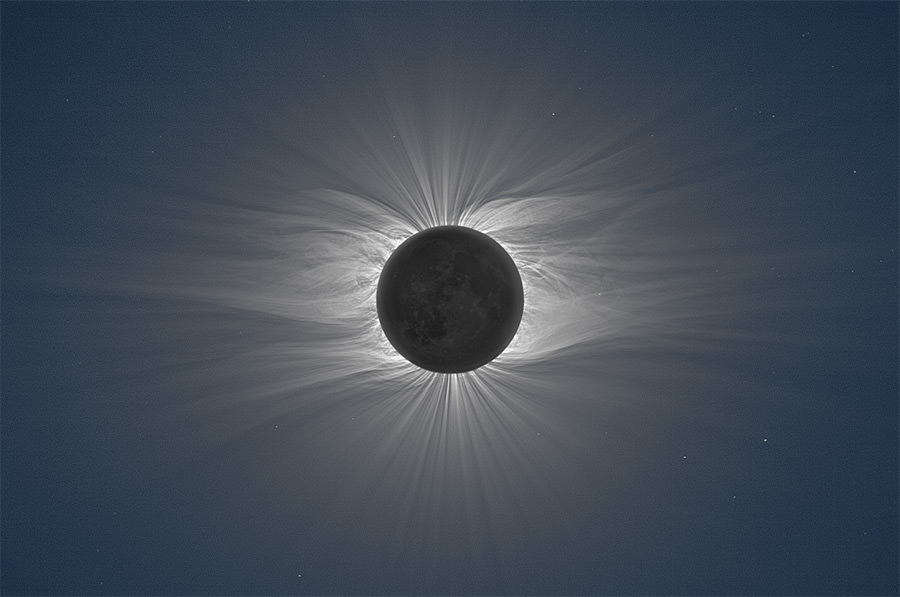
\includegraphics[scale=0.45]{images/solar_eclipse}
\caption[White-light corona during an eclipse]{The white-light corona during a solar eclipse. Occultation of the bright solar disk by the moon reveals the faint outer atmosphere of the Sun, known as the corona. It is highly structured, showing features such as streamers and plumes. {\it Eclipse photograph courtesy of Miloslav Druckm\"{u}ller \href{http://www.zam.fme.vutbr.cz/~druck/Index.htm}{http://www.zam.fme.vutbr.cz}}}
\label{fig:seclipse}
\end{center}
\end{figure}
This is known as the white-light corona and is due to scattering of photospheric light by coronal particles. Of particular interest here is the K-corona (as first introduced in Section~\ref{sec:123}); this is the corona that is visible because of Thomson scattering of photospheric light by free electrons. 
Before the early 20th century the only way to view the corona was for a short period during a solar eclipse when the moon blocks direct photospheric light. Under normal conditions direct sunlight overwhelms the faint corona. In 1939 the French astronomer Bernard Lyot developed a telescope, known as a coronagraph, which allowed observation of the corona at any time \citep{lyot1939}. A coronagraph is an optical system that provides an artificial eclipse of direct photospheric light so the much fainter corona can be imaged. a description of Lyot's original design, and the space based instruments based on this design, is given here.
%A coronagraph is an optical system that provides an artificial eclipse so the faint corona may be imaged at any time. The first working coronagraph was invented by the French astronomer Bernard Lyot in 1930.

\subsection{Lyot Coronagraph}\label{sec:22}
A basic schematic of the Lyot coronagraph is given in Figure~\ref{fig:lyot}. The objective lens O1 forms an image of the solar disk onto
to the internal occulting disk D1 (a metal cone), where the light is reflected away from the field lens O2. Lyot's key invention was the Lyot stop (A1) and Lyot spot (D2). The field lens O2 images the aperture A0 and its diffraction pattern onto the Lyot stop. If the Lyot stop were not there, this light would reach the focal plane and contaminate the image. The Lyot spot (D2) blocks spurious light caused by multiple reflections in the field lens O2. It also blocks any light diffracted by the occulter D1. In theory, the only light that is transmitted through the system is that coming from beyond the solar disk. This light is focused onto the image plane F by O3. In practice there may be undesired and excess light that is transmitted through the system and great care is taken to reduce this as much as possible. The Lyot coronagraph is described as internally occulting due to the placement of the occulting disk behind the first objective lens. This is to distinguish it from a externally occulted system in which an extra disk is placed in front of the objective lens. The externally occulted coronagraph prevents photospheric light from entering the optical system in the first place, thus allowing much fainter objects to be imaged. However, the external occulter prevents imaging of the very low corona. Hence there is a choice between very low contaminant light levels in the telescope or imaging of the low corona. 

All coronagraphs inherit their basic design from Lyot's original, and a number of these are space based instruments providing observation of the corona over many height ranges.

\begin{figure}[!t]
\begin{center}
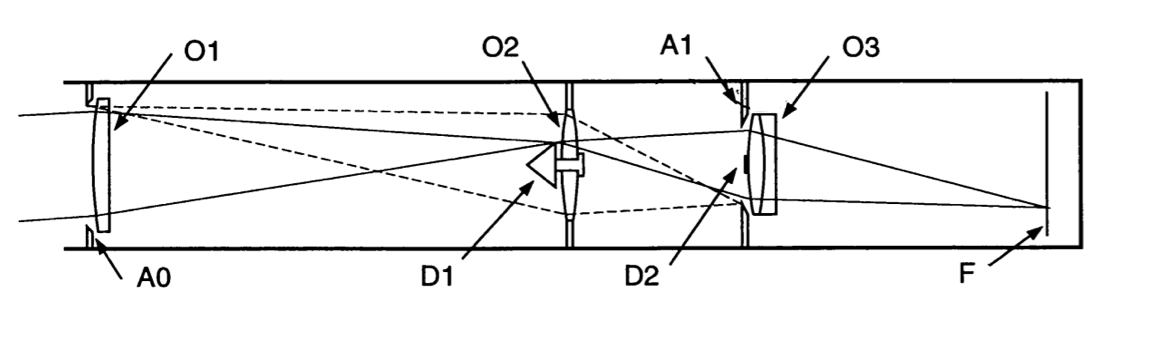
\includegraphics[scale=0.35, trim=0.0cm 2cm 0cm 2cm]{lyot.png}
\caption[The Lyot coronagraph]{A schematic of the basic optical design of the Lyot coronagraph. Lyot's key inventions where the placement of a Lyot stop (A1) and Lyot spot (D2) at the positions where diffracted light would contaminate the image and obscure the faint corona.}
\label{fig:lyot}
\end{center}
\end{figure}

\subsubsection{SOHO LASCO}\label{sec:23}

The Solar and Heliospheric Observatory (SOHO) is located at Lagrangian point 1 and carries a suite of in-situ and remote sensing instruments, including three coronagraphs collectively known as the Large Angle Spectrometric Coronagraph (LASCO) \citep{bru95}. LASCO comprises three different coronagraphs, C1, C2, and C3, that were built to observe the corona over heliocentric distance range of 1.1--30\,$R_{\odot}$. 

C1 is a reflector version of the internally occulted Lyot coronagraph that images the corona over a distance range of 1.1--3\,$R_{\odot}$. A tunable Fabrey-Perot interferometer is placed after the Lyot stop to allow narrow passband images of the solar corona at the lines of Fe\,\rmnum{14}, Ca\,\rmnum{15}, Na\,\rmnum{1}, Fe\,\rmnum{10}, and H$\alpha$.
C1 operates a $1024\times1024$ CCD with a pixel size of $5.6''$, giving a spatial resolution of $\sim11''$. The Rayleigh diffraction limited resolution of the telescope if $3.3''$ at $530.3$\,nm. Unfortunately C1 failed in 1997 and is no longer in operation. 
\begin{figure}[!t]
\begin{center}
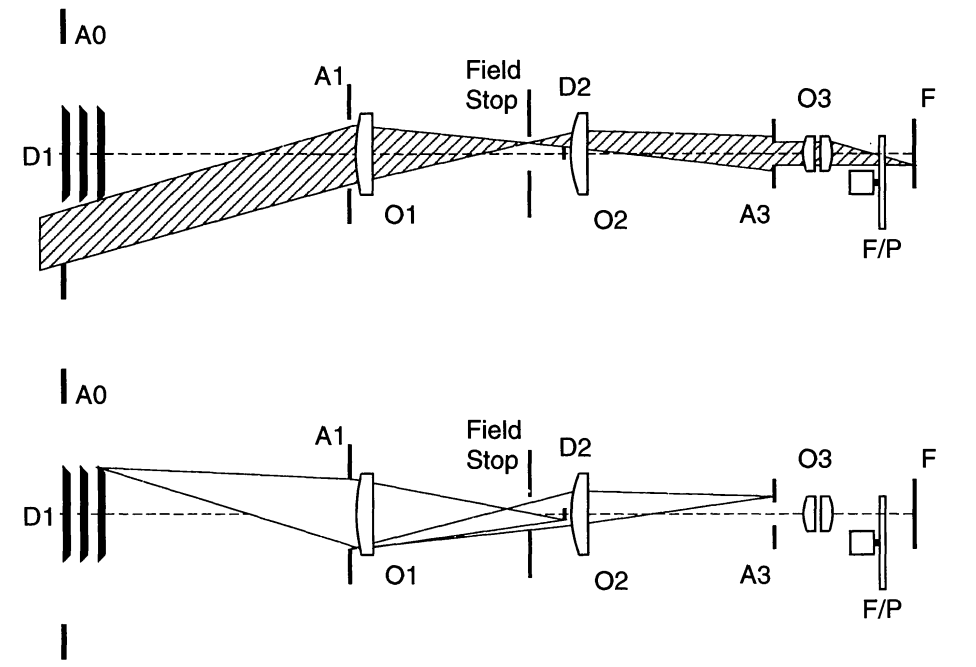
\includegraphics[scale=0.4]{c2_concept.png}
\caption[The LASCO C2 coronagraph optics]{Conceptual optical layout of the LASCO C2 corongraph. The top ray-tracing diagram shows the image formation, while the bottom diagram demonstrates the stray light supression and occultation \citep{bru95}.}
\label{fig:c2_concept}
\end{center}
\end{figure}

C2 is an externally occulted, broadband, refractor coronagraph that images the corona from 1.5--6$\,R_{\odot}$\footnote{The levels of stray-light just beyond the occulter mean that in practice the C2 inner field of view limit is $2.2\,R_{\odot}$}. The conceptual diagram for its optical layout is shown in Figure~\ref{fig:c2_concept}. The front aperture A0 is on the left of the diagram and includes the external occulter D1, consisting of three consecutive circular disks on a common spindle, these disks completely shadow the entrance aperture A1 from direct sunlight. The disks also successively intercept diffracted sunlight from the one before to minimize the total diffracted light from the solar disk falling on the object lens O1. 
\begin{figure}[!t]
\begin{center}
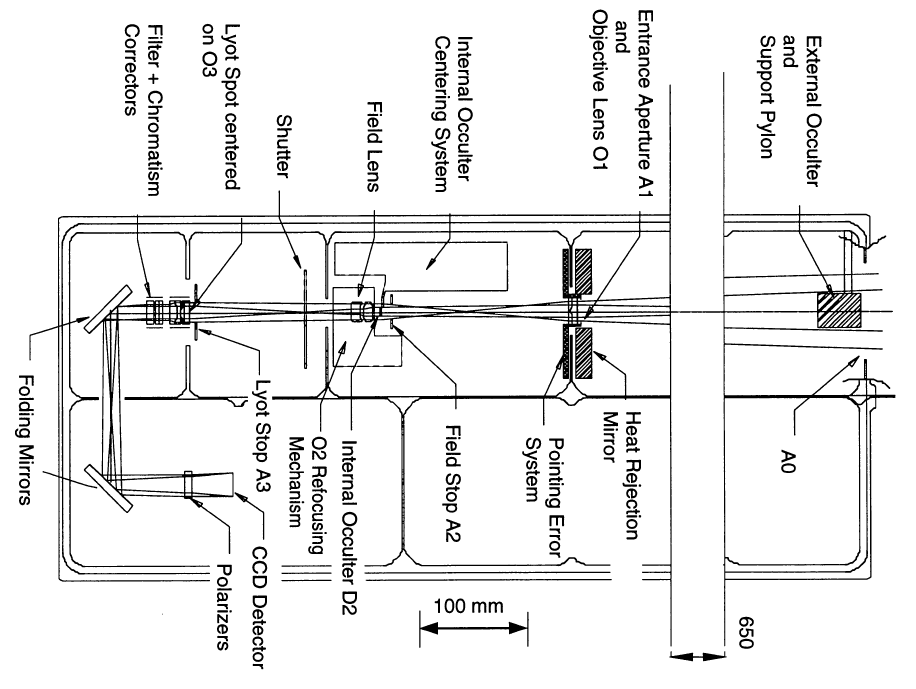
\includegraphics[scale=0.5, angle=90]{c2_detail.png}
\caption[The LASCO C2 coronagraph detail]{A detailed layout of the C2 coronagraph optics and mechanical construct \citep{bru95}.}
\label{fig:c2_detail}
\end{center}
\end{figure}
The disks have fine threads on their edges that have been diamond machined, and have a cone opening angle that is slightly bigger than the solar disk at L1 ($32.31'$). This ensures a very high level of light rejection at the external occulter. The objective lens O1 images the corona at the field stop, which sets the outer limit to the field of view of the telescope ($5\,R_{\odot}$ for C2). O1 also images D1 onto the D2 internal occulter, which also serves to intercept any residual stray light diffracted at D1. The lens O2 collimates the coronal image and also images the entrance aperture A1 onto the Lyot stop A3. Finally the lens O3 images the corona onto the focal plane F. The combination of the internal and external occulters, the aperture stops, and a heat rejection mirror at the entrance aperture (Figure~\ref{fig:c2_detail}), mean that the the coronagraph has stray light levels that are an order of magnitude improvement over previous space based coronagraphs e.g., stray light levels are typically an order of magnitude or more lower than the coronal brightness, allowing the detection of features in the range of $2\times10^{-7}$--$15\times0^{-10}\,\mathrm{B}_{\odot}$ where $\mathrm{B}_{\odot}$ is mean solar brightness (MSB) unit \citep{bru95}.

The light focused onto the focal plane by the O3 lens first passes through a colour filter and polarizer wheel, which selects the band pass and takes three polarization images at $0^{\circ}$, $-60^{\circ}$ and $+60^{\circ}$ such that total or polarized brightness images of the corona may be taken. Mounted at the focal plane is a front-side illuminated $1024\times1024$ CCD, with $21\mu$ square pixels (equivalent angular size if $11.4''$),  operating in a nominal spectral range of $500-700$\,nm, at a temperature of $-80^{\circ}$\,C. CCD readout takes approximately 22 seconds, after which the image may be compressed by a number of algorithms before being sent to the ground station. Among the observing nominal modes are routine flat-field exposures and dark current exposures to be used in calibration. At current operations the C2 coronagraph offers a total brightness image of the corona every 15 minutes.  

Finally, C3 is an externally occulted broadband lens coronagraph that images the corona from 3.7--30$\,R_{\odot}$, with a pixel size of $5'6'$ and brightness range of $3\times10^{-9}$--$1\times10^{-11}$. It has the same optical design as C2 (Figure~\ref{fig:c2_concept}).

The C1, C2 and C3 coronagraph data is processed on-board using a number of steps that may compress the data before transmission to an Earth ground station. Each telescope feeds its compressed data to the same telemetry buffer which can store up to 2\,Mb. The  LASCO telemetry rate is 4.2\,kb\,s$^{-1}$ and communication with the ground is via the Deep Space Network (DPS). The SOHO spacecraft is usually in contact with the DPS for approximately 2 hours per day. Data captured by the DPS is then transmitted to servers at NASA's Goddard Space Flight Centre (GSFC) and the Naval Research Laboratory (NRL). Only the C2 coronagraph is used in this thesis, and some sample level-2 data for C2 is shown in Figure~\ref{fig:lasco_c2_obs}
\begin{figure}[!t]
\begin{center}
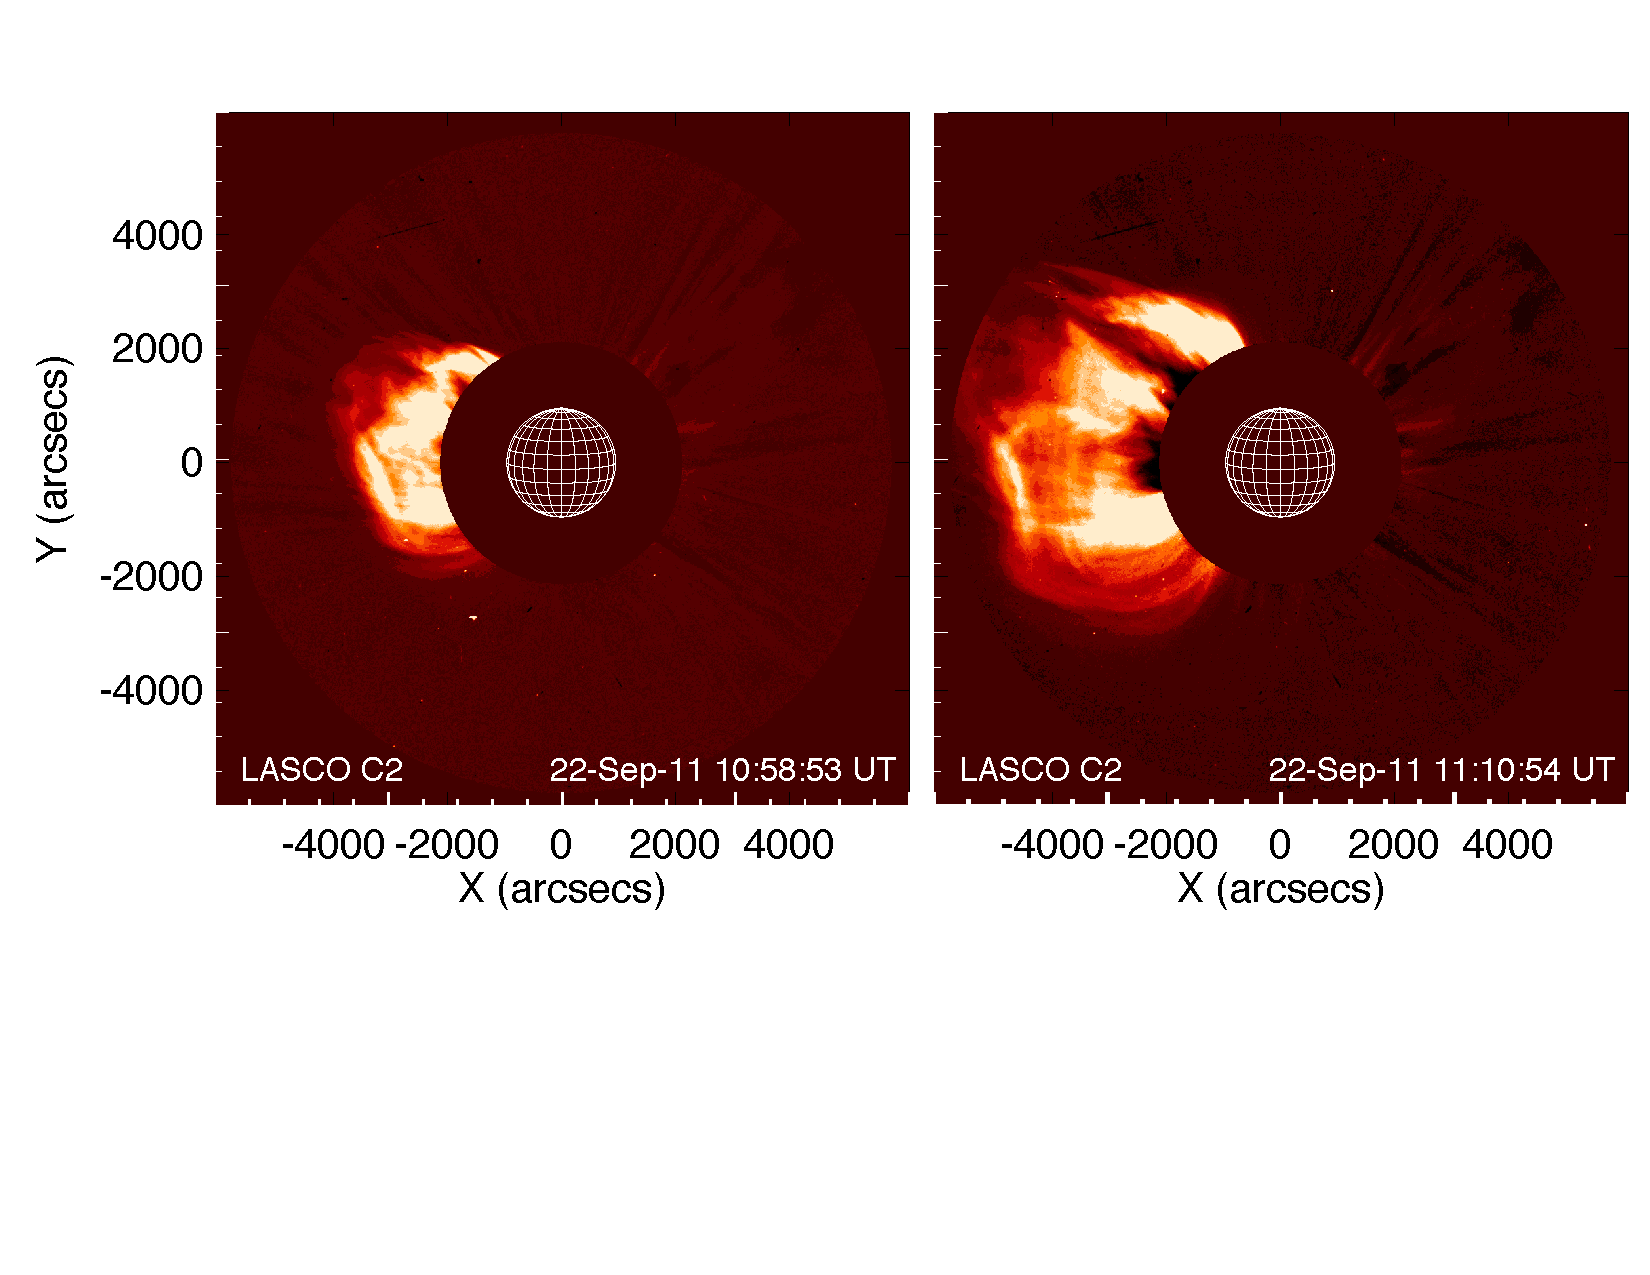
\includegraphics[scale=0.55, trim=2cm 6cm 1cm 2cm]{images/lasco_c2_thesis.pdf}
\caption[LASCO C2 Observations]{LASCO C2 Observations of a CME occurring on 22 September 201. The central disk is from the occulter. A heliographic grid is over-layed to show the size of the sun.}
\label{fig:lasco_c2_obs}
\end{center}
\end{figure}


\subsubsection{STEREO COR1 and COR2}\label{sec:22}
The \emph{Solar Terrestrial Relations Observatory} \citep[\emph{STEREO};][]{kai08} Ahead and Behind are two nearly identical spacecraft traveling ahead and behind Earth in its orbit. Each spacecraft is receding from Earth at a rate of $\pm22^{\circ}$ per year, such that they are effectively traveling around the Sun in opposite directions. For the spacecraft locations at three different times see Figure~\ref{fig:where_str}. They carry an identical set of instruments known as the Sun Earth Coronal Connection and Heliospheric Investigation (SECCHI) suite, including in situ detectors and a variety of imagers.
\begin{sidewaysfigure}
\centering
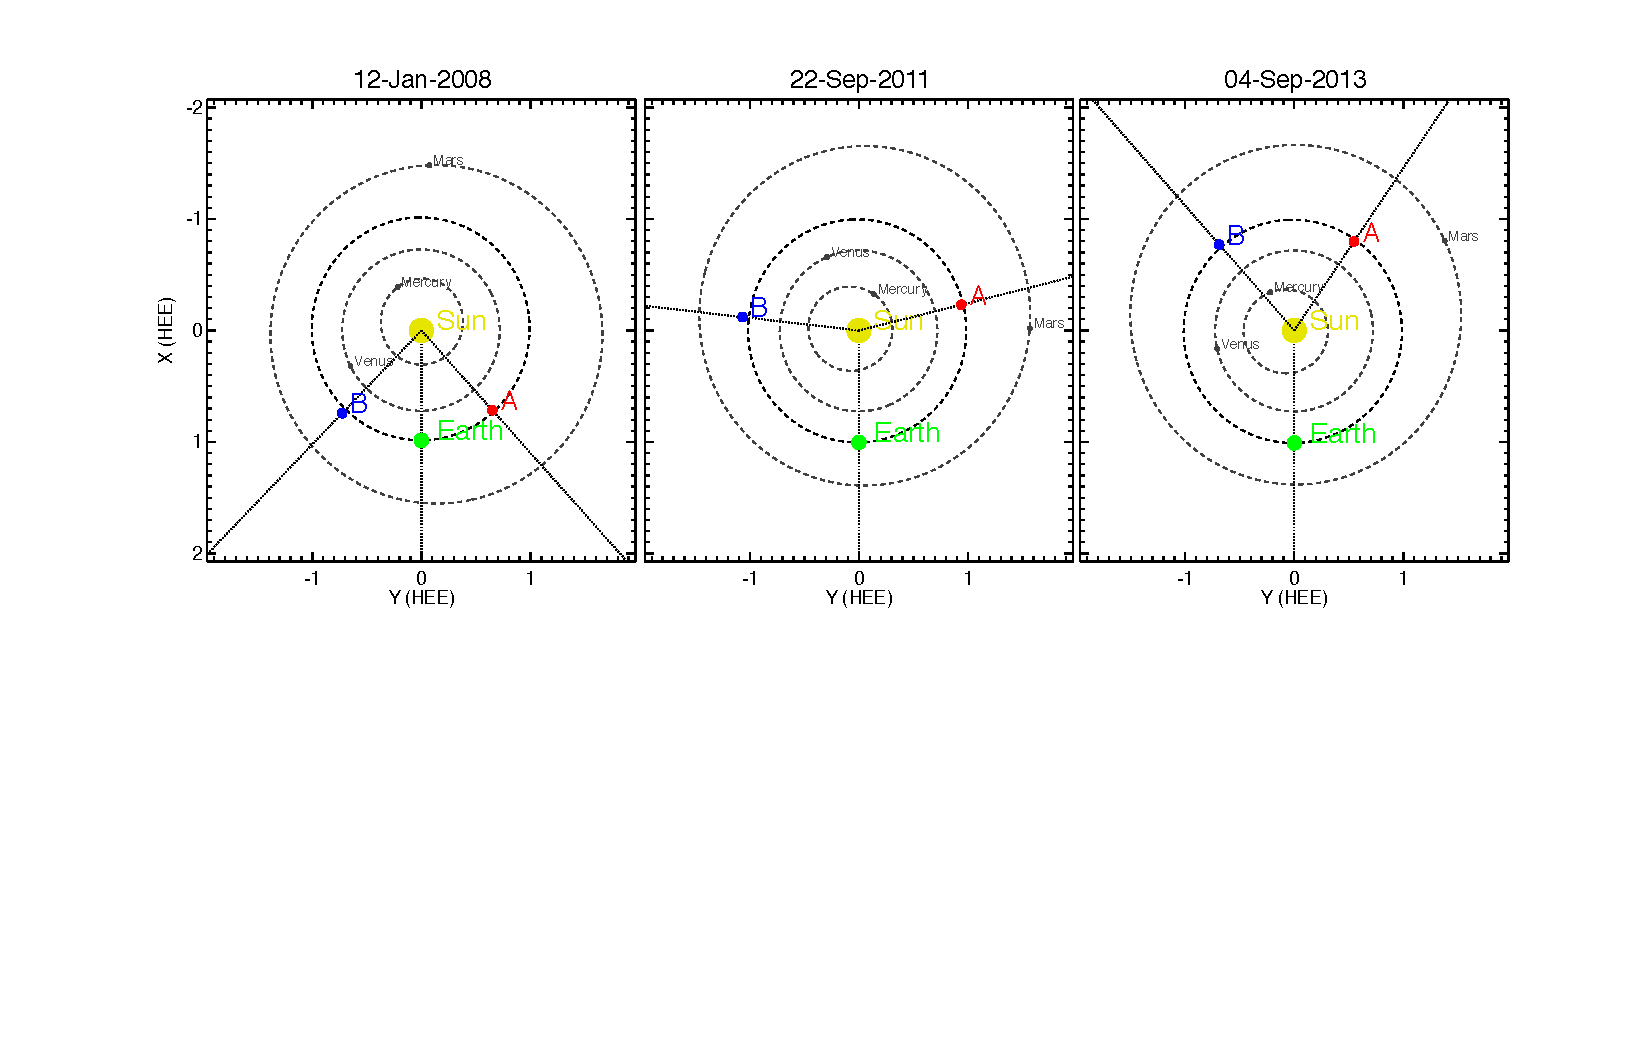
\includegraphics[scale=0.9, trim=2cm 7cm 0cm 0cm]{where_stereo_thesis.pdf}
\caption[STEREO spacecraft positions]{The {\emph STEREO} A and B spacecraft positions with respect to Sun, Earth and inner planets.}
\label{fig:where_str}
\end{sidewaysfigure}
On each spacecraft there are two coronagraphs, COR1 and COR2 \citep{how08}. The Ahead COR1 and COR2 combined with Behind COR1 and COR2 offer a stereoscopic view of the corona and any transient event taking place, such as a CME.
\begin{figure}[!t]
\begin{center}
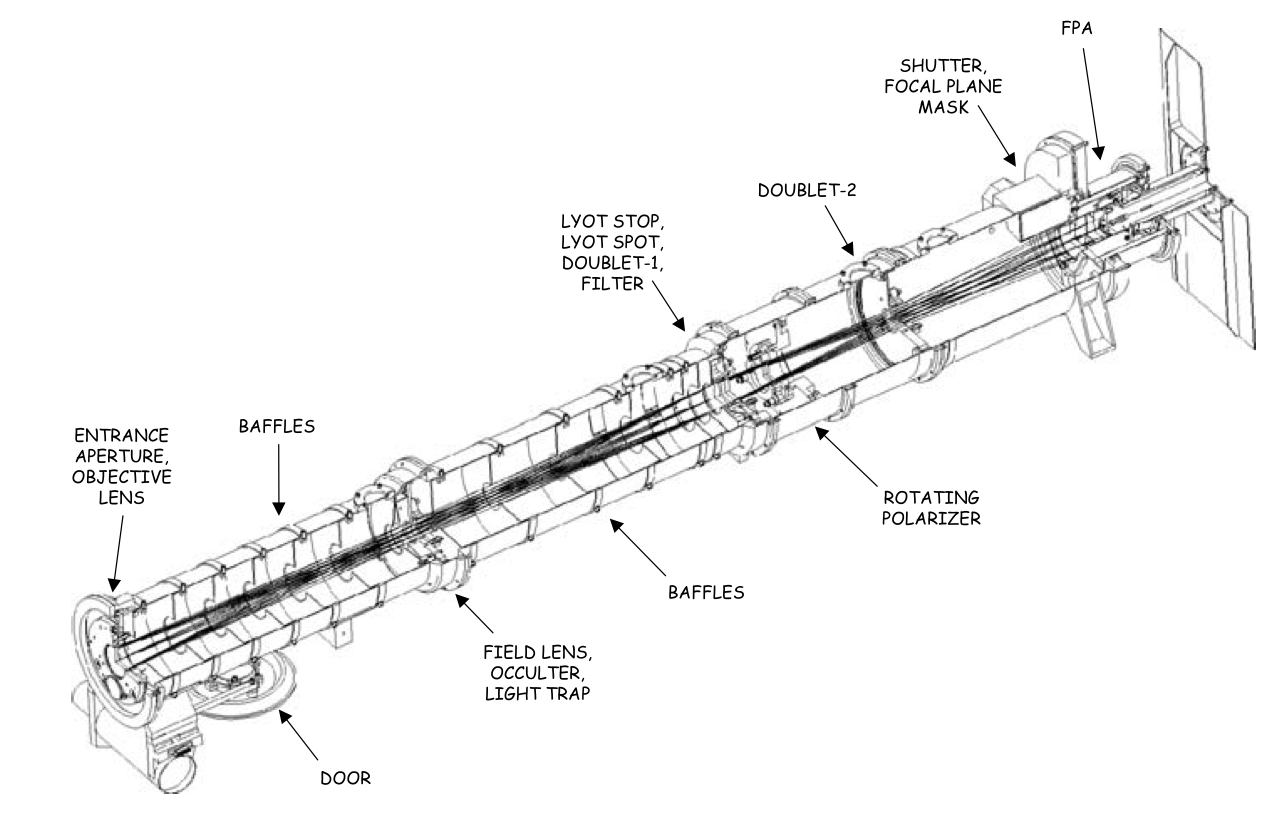
\includegraphics[width=0.8\textwidth]{images/COR1_design}
\caption[The COR1 coronagraph]{A schematic of the basic optical design of the the COR1 coronagraph. There are two such identical instruments, one on the Ahead and one on the Behind spacecraft. It is the same basic design as the Lyot coronagraph with the addition of baffles to prevent scattered light and a polarizer behind the Lyot stop \citep{thomp2008}.}
\label{fig:COR1_design}
\end{center}
\end{figure}
\begin{figure}[!t]
\begin{center}
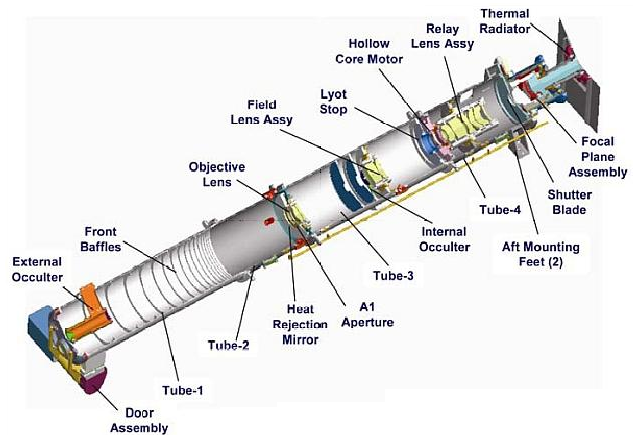
\includegraphics[width=0.8\textwidth]{images/cor2}
\caption[The COR2 coronagraph]{A schematic of the basic optical design of the COR2 coronagraph. This is an externally occulted coronagraph, meaning it has an extra occultation disk in front of the objective lens. This results in less internally scattered light, but also results in an obscuration of the inner corona. As with COR1, there are two such identical instruments, one on the Ahead and one on the Behind spacecraft \citep{how08}.}
\label{fig:cor2}
\end{center}
\end{figure}


COR1 is an internally occulted Lyot refractive coronagraph (Figure~\ref{fig:COR1_design}) and derives its basic design from Figure~\ref{fig:lyot}. It images the inner corona with a field of view from 1.4--4.5\,$R_{\odot}$, centered on the H$\alpha$ line at 656\,nm with a 22.5\,nm wide passband. 
It has an internal polarizer located after the first doublet lens in the optical system (Figure~\ref{fig:COR1_design}) and takes three images at $0^{\circ}$, $\pm60^{\circ}$, so that polarized or total brightness images of the inner corona may be produced. Stray light levels of both COR1 A and B lie between 0.1--1$\times10^{-6}\,\mathrm{B}_{\odot}$, and some defects in the field lens can cause ring shaped features with 1.4$\times10^{-6}\,\mathrm{B}_{\odot}$ \citep{how08}. The focal plane of the instrument has a $1024\times1024$ pixel CCD, with a platescale of 3.75$''$ per pixel \citep{thomp2008}. To improve the signal to noise, a $2\times2$ pixel binning may be performed. A typical observing sequence will perform three 1 second exposures (one for each polarization state at 0$^{\circ}$, -60$^{\circ}$, and +60$^{\circ}$), in total taking 11 seconds. Typical CCD read-out times result in an image sequence cadence of 8 minutes (time between a three image set and the next three image set).
\begin{figure}[!t]
\begin{center}
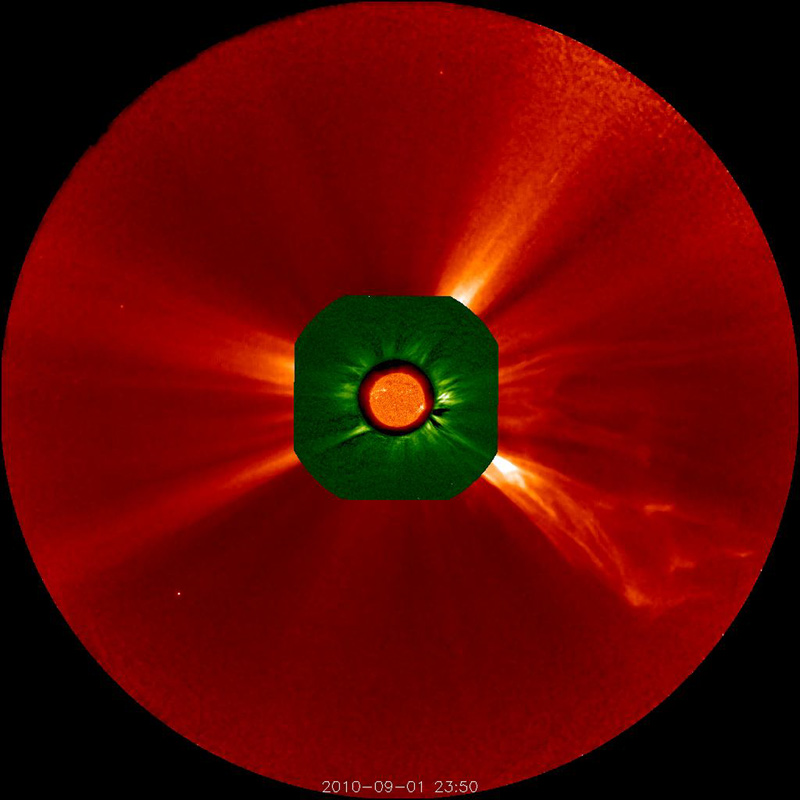
\includegraphics[scale=0.4]{euvi_cor1_cor2.png}
\caption[COR1 and COR2 observations]{Observation of the corona from the COR1 (green), and COR2 (red) coronagraphs on board the STEREO Ahead spacecraft, 01 Sep 2009 23:50 UT. An Extreme Ultraviolet Imaging (EUVI) 304\,\AA~ image of the sun is shown at the center. A CME was observed, erupting to the south-west. {\it Image Courtesy of Alex Young, http://www.thesuntoday.org/.} }
\label{fig:cor1cor2}
\end{center}
\end{figure}

COR2 is an externally occulted Lyot coronagraph and derives much of its design from the LASCO C2 and C3 coronagraphs. Externally occulted coronagraphs have an extra occulting disk in front of the objective lens, see Figure~\ref{fig:cor2} or Figure~\ref{fig:c2_concept}. As described, a downside to this design is that the external occulter does not allow the inner corona to be imaged, hence such coronagraphs are usually used to observe the extended corona to larger heights. The COR2 inner edge field of view limit is defined by the external occulter, while the outer edge is determined by the field stop, resulting in a field of view from 2.5--15$\,R_{\odot}$. The filter used in the assembly has a bandpass of 650--750\,nm at FWHM. The focal plane contains a back-lit CCD that nominally produces $2048\times2048$ images, with 14.7$''$ per pixel. Like COR1 it has an internal polarizer producing three linearly polarized images per observing sequence (30 minutes).

These white light imagers of the corona allow for a stereoscopic view of CMEs in a total field of view covering 1.4--15\,$R_{\odot}$. The two viewpoint capabilities of these telescopes offer a more accurate observational estimation of both CME kinematics and CME mass, resulting in a better understanding of CME dynamics. A sample observation using COR1 and COR2 from the Ahead spacecraft is shown in Figure~\ref{fig:cor1cor2}


\subsubsection{Whilte-light Image Data Reduction}

All coronagraph images, including those produced by COR1, COR2, and the LASCO coronagraphs, have a number of basic image processing steps in common. The amount by which the data has been processed is described in terms of `levels', with the most basic raw data product of the telescope being level-0. Level-0 usually comprises the compressed data that comes directly from the spacecraft telemetry stream via the DPS. The data is processed from level-0 to level-0.5 by decompressing the spacecraft data and re-packaged into flexible image transport system (FITS) files, which is an open standard format for all astronomical images. 

Calibration of the data into a scientifically usable format results in level-1 data. The steps to produce level-1 data are as follows:
\begin{itemize}
\item Darks current image subtraction. Each CCD will carry some level of residual voltage even when the camera shutter is closed. This residual voltage is due to the thermal energy of the electrons in each well of the CCD. The voltage (thermal energy) must be removed from the image since it is not due to light from an observed source. The `dark image' is taken with the camera shutter closed and an exposure performed as normal (exposure time the same as the raw image). The dark image is simply subtracted from the raw image
%
\item Bias image subtraction. Similar to dark current the CCD will have some charge due systematic defects. These are usually exposed by taking an image with the shutter closed and for the shortest possible exposure times. They bias image is also subtracted from the raw image.
%
\item Flat field correction. Every CCD will have a non-uniform response across its photon collecting area. One side of the CCD, or any arbitrary grouping of pixels, may naturally be more sensitive than the other pixels. As well as this, the optical system itself may produce some brightness variation across the focal plane. To account for this, the raw image must be divided by a `flat-field' in order to normalize the spatially non-uniform response detected by the CCD. The `flat-field' is an image taken of a uniformly illuminated surface. For space based telescopes this uniformly illuminated image is usually taken by closing the telescope front aperture and lighting a lamp placed near the aperture cover, or the telescope front door may contain a `diffuser' that scatters sun light to provide uniform illumination. The LASCO system uses a quartz filter on the telescope cover that diffuses exterior light, allowing a uniform illumination of the CCD \citep{bru95}. It is important that the dark current and bias images be subtracted from the flat-field before the raw images (which are also dark and bias image subtracted) is divided by the flat field.
%
\end{itemize}
Accounting for dark current, bias, and flat-fielding are the most fundamental of all CCD imaging calibration routines. They can be summarised as
\begin{equation}
I_{cal}(x_i, y_i) = \frac{ I_{raw}(x_i, y_i)  - I_{dark}(x_i, y_i) - I_{bias}(x_i, y_i)  }{ | I_{flat}(x_i, y_i) - I_{dark}(x_i, y_i) - I_{bias}(x_i, y_i)| }
\end{equation}
where $I$ are the images, $(x_i, y_i)$ are pixel coordinates, and the $|~|$ in the denominator mean that the dark and bias subtracted flat-field is normalized (divided by itself). Other standard techniques beyond the most basic ones include
\begin{itemize}
%
%
\item Vignetting. All camera imaging systems suffer from vignetting, a reduction in brightness at the edge of the field of view. In coronagraph systems this is particularly important since a vignette can occur at the inner field of view, due to the occulting disk and also due to the pylon supports of the disk. Special vignetting calibration images are performed to account for this effect; they are used to normalise the image in the same way as the flat-field is performed.
%
%
\item De-warping. The image may suffer some geometric distortions due to a deformity in an one of the numerous optical components of the telescope. This may result in the image being warped. Pre-flight experiments completely characterize any optical distortion so that all raw image may be `de-warped'
%
%
\item Brightness calibration. This is the conversion from CCD data numbers per second (DN\,s$^{-1}$) to physical measures of intensity e.g., mean solar brightness (MSB) units (1 MSB = $2.01\times10^{10}$\,ergs\,s$^{-1}$\,cm$^{-2}$\, sr$^{-1}$). The conversion factors may be calculated in a pre-flight lab, or during inflight via observations of objects with known intensities. Mercury, Venus, or Jupiter have served as calibrators for COR\,1 and 2 \citep{thomp2008}.
\end{itemize}
The above steps are the most frequently taken to ensure clean and calibrated astronomical images. They apply to every telescope using a CCD imaging system and every telescope type, including ground and spaced-based systems. For the coronagraphs mentioned above, the steps are performed on each polarization image separately before summing to total or polarized brightness using the following equations
\begin{eqnarray}
B &=& \frac{2}{3}(I_0 + I_{+60} + I_{-60}) \\
pB &=& \frac{4}{3}\sqrt{(I_0 + I_{+60} + I_{-60})^2 - 3(I_0I_{+60} + I_0I_{-60} + I_{-60}I_{+60}) )}
\end{eqnarray}
adapted from \citet{billings1966}. $I$ are the intensity values in each pixel and the 0$^{\circ}$, $+60^{\circ}$, and $-60^{\circ}$ represent the three polarizations states e.g., the polarizations states of COR 1 and 2.

Anything beyond the above calibration steps is termed level-2 and is usually instrument specific or specific to the scientific goal. Chapter 4 will discuss the production of `mass images' where the pixel values have units of grams, this may also be termed level-2 processing.


\section{Ultraviolet Observations}\label{sec:4}

\subsection{The Atmospheric Imaging Assembly}\label{sec:40}

The Atmospheric Imaging Assembly (AIA), on board NASA's Solar Dynamics Observatory (SDO), consists of four Cassegrain telescopes that provide visible, ultraviolet (UV), and extreme ultraviolet (EUV) full-disk images of the transition region and corona up to $0.5\,R_{\odot}$/ with 1.5" spatial resolution and 12-second temporal resolution \citep{lemen2012}. The telescopes provide imaging in seven extreme ultraviolet passbands centered on the lines Fe\,\Rmnum{18} \,(94\,\AA), Fe\Rmnum{8}, \Rmnum{21}\,(131\,\AA), Fe\Rmnum{9} \,(171\,\AA), Fe\Rmnum{12}, \Rmnum{24}\,(193\,\AA), Fe\Rmnum{14}\,(211\,\AA), He\Rmnum{2}\,(304\,\AA), Fe\Rmnum{16}\,(335\,\AA). One of the telescopes observes longer wavelengths at C\Rmnum{4}\,(1600\,\AA), the nearby continuum ay (1700\,\AA) and a broadband visible filter centered on (4500\,\AA)  giving a full temperature coverage of $6\times10^4$\,K to $2\times10^7$\,K.

Each telescope has a field of view is 41' circular diameter, a 20\,cm primary mirror and an active secondary mirror that is pointed in response to signals from a guide telescope. 
\begin{figure}[!t]
\begin{center}
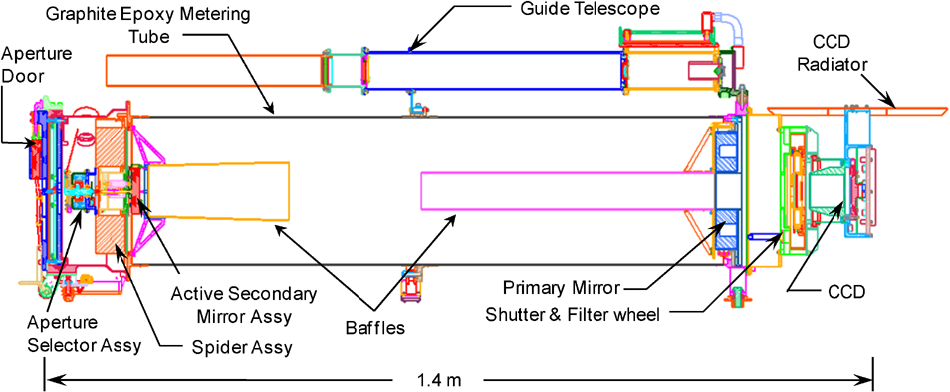
\includegraphics[scale=1.1]{aia_telescope.png}
\caption[The AIA telescope design]{The Atmospheric Imaging Assemly (AIA) telescope design. AIA employs for these Cassegrain type telescopes, with telescope 1, 2 and 4 serving as dual channel passbands, and telescope 3 permitting imaging at three separate passbands \citep{lemen2012}.}
\end{center}
\end{figure}
Each mirror is polished to a roughness of $<5\,\AA$~rms in the spatial frequency range $10^{-3}-5\times10^{-1}$\,nm$^{-1}$. The telescopes are dual channel i.e., the mirrors in each telescope have two different multi-layer coatings on either half so as to be reflective at a single desired central wavelength on one half. For example, half of mirror 2 has a peak reflectance at 195.5\,\AA with the other half reflects at 211.3\,\AA. These two-channel combinations for each mirror in all four telescopes is shown in Figure X. Half of mirror 3 provides the broadband UV and visible channel, with a coating that gives the ability to reflect at 1600, 1700, and 4500\,\AA, while the other half of the mirror provides the optics for the 171\,\AA channel. Hence telescope 3 provides the optics for four different bandpasses. 

Metal entrance filters at the aperture of each telescope, combined with a filter wheel located in front of each focal plane, suppress unwanted UV, visible, and IR radiation. The filters are either made of aluminium, used for wavelengths of 171\,\AA~or longer, and zirconium used for the shorter 94\,\AA and 131\,\AA wavelengths. Telescope 3 has an aluminium (for 171\,\AA)and MgF$-2$ (for the UV broadband)entrance window and 3 different filters on the filter wheel that cater for observation in 171\,\AA~(aluminium), 1600\,\AA~(MgF$-2$), 1700\,\AA~and 4500\,\AA~(fused silica). A mechanical shutter regulates exposure time to nominal short exposure times of 5\,ms and nominal long exposure times of 80\,ms. Flight software can also select any custom exposure time.
\begin{figure}[!t]
\begin{center}
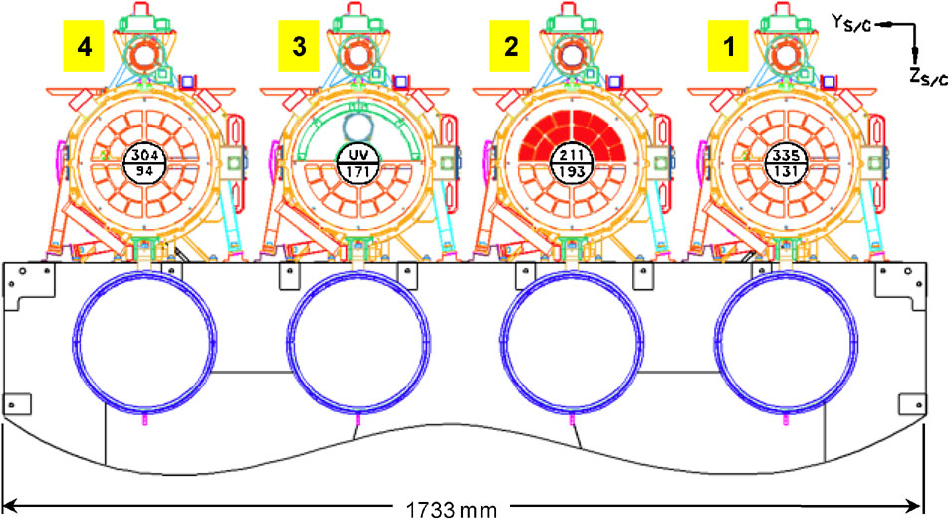
\includegraphics[scale=1.2]{aia_4telescopes.png}
\caption[The four telescopes of AIA]{The four telescopes making up the Atmospheric Imaging Assembly (AIA) \citep{lemen2012}.}
\end{center}
\end{figure}
The focal plane of each telescope contains a back-illuminated $4096\times4096$ pixel CCD, with each square pixel having a 12\,$\mu$m size. Each CCD is read out in 4 quadrants, via an amplifier, into a camera box with four interfaces (one for each quadrant). Each quadrant is read out at a rate of 2\,Mpixels\,s$^{-1}$ and data transmission to the on-board computer occurs at a rate of 100\,Mb\,s$^{-1}$
\begin{figure}[!t]
\begin{center}
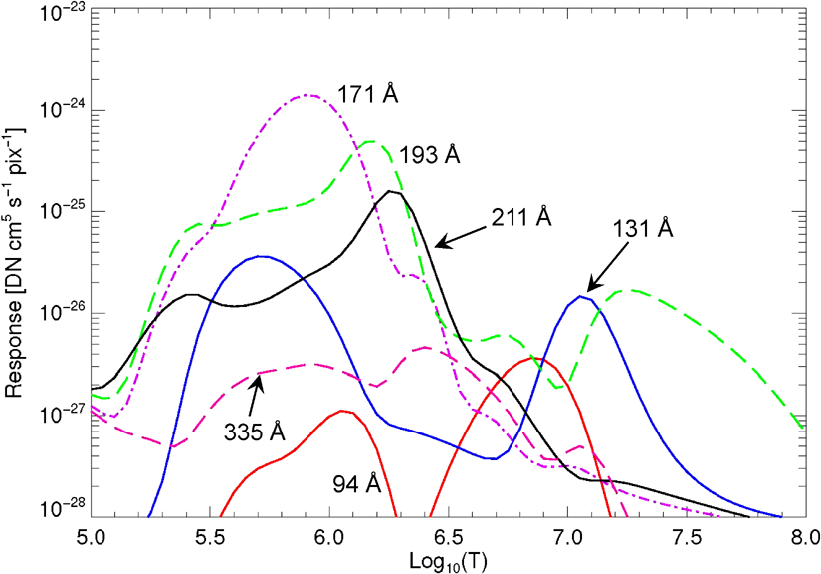
\includegraphics[scale=1.2]{aia_passbands.png}
\caption[AIA temperature response]{The Atmospheric Imaging Assembly temperature responses for each of its passbands. The passbands cover temperatures that include the transition region, to quiet corona, to flaring corona. The 4500\,\AA~ passband is not shown here, it's temperature coverage results in photospheric imaging. \citep{lemen2012}.}
\end{center}
\end{figure}
All of the steps above described for white-light calibration are relevant for ultraviolet CCD imaging also. The AIA calibration procedure to bring the data from level-0.5 to level-1 include de-biasing, dark subtraction, flat-fielding, de-vignetting, de-warping, and brightness calibration. Some example images of AIA are shown in Figure~\ref{fig:aia_corona}

\section{Radio Observations}\label{sec:3}

\subsection{Nancay Radioheliograph}\label{sec:33}

Radio images of the solar corona are important to probe both quiet activity and also flaring an eruptive activity. As described in Section 2.X, flaring and eruptive activity may often result in high speed electrons which can excite plasma emission and gyrosynchrotron emission. The Nan\c{c}ay Radioheliograph is a solar-dedicated radio interferometer located at Nan\c{c}ay, central France ($47^{\circ}$N~$2^{\circ}$E), that observed such activity at ten frequencies between 150 and 450\,MHz \citep{kerdraon1997}.
\begin{figure}[t!]
\begin{center}
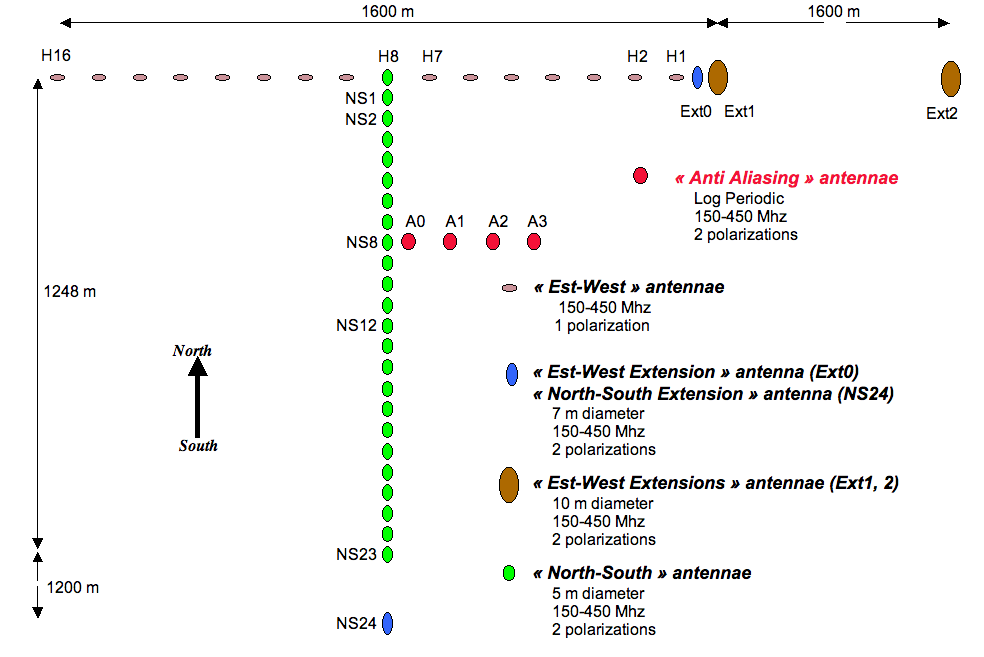
\includegraphics[scale=0.55, angle=90]{nrh_layout}
\caption[The Nancay Radioheliograph layout]{The Nancay Radioheliograph layout}
\end{center}
\label{fig:eclipse}
\end{figure}

The array antennas are arranged in a perpendicular \textquoteleft T' shape. The east west array consisting 19 antennas providing baselines in the range of 50\,m to 3200\,m. Four these antennas have parabolic collectors with four orthogonal thick dipole feeds at the focus providing two orthogonal polarizations in the 150-450\,MHz band. The remaining 15 have no collectors (no dishes) and consist only of thick dipole antennas providing linear polarization only. The north-south array consists of 24 five meter dishes with wide band feeds, covering baselines between 54 to 1248\,m. The antenna front end electronics include low noise high dynamic range (45\,dB) pre-amplifiers, band filters for frequency switching and a local oscillator which mixes the signal 113\,MHz before it is sent to the receiver \citep{avignon1989}. At the receiver the signal is further mixed down to 10.7\,MHz and fed through a bandpass filter of 700\,kHz width (final bandwidth of each observed frequency), digitized and sent to the correlator.

%Mark II: monofrequency east-west (169 MHz)
%Mark III: monofrequency east-west and north-south (169 MHz), receiver has 45 dB dynamic range (Bonmartin 1983)
%Mark IV: multifrequency (5) on north-south (150-450 MHz), monofrequency on the east-west (164 MHz) (Avignon 1989)
% Multifrequency (5) on north-south and east-west baslines (150-450 MHz) (1993 AdSpR)
%Present: multifreqquency (10) on north-south and east-west baselines (150-450 MHz), digital correlator added (Kerdraon 1997)

The original array consisted of only the east-west baselines, with the north-south being added later in the early 1980s \citep{bonmartin1983}, hence the two separate arrays operate off different correlators. The visibility outputs of each correlator are digitized by sampling every 5\,ms, resulting in 4 images every 5\,ms (Stokes I and V for the east-west and north south arrays), with a down sampling of by integrating at least 4 successive images in order to ease storage loads \citep{avignon1989}. These images are only 1D, offering projected intensity profiles along two axes. Originally, full 2D maps were created by Earth rotation synthesis using the standard 1D observations over one entire day \citep{nrh1993}. Such limitations were mainly due to the use of an analog correlator. However, a digital correlator installed in 1997 now provides fast 2D images using the most westerly 17 antennas of the east-west baseline \citep{kerdraon1997}, resulting in a spatial resolution that is 4 times lower than the 1D east-west images. Systematic daily observations of 2D images are usually performed at between 0.1 and 1 image per second.

All radio interferometers measure a property known as visibility, which is the Fourier transform of the observed sky brightness distribution
\begin{equation}
V(u,v)=\int I(l,m)\mathrm{exp}(i2\pi[ul +vm])dldm
\end{equation}
where $V$ is the visibility, $(u,v)$ are the spatial frequency of fringes on the sky, corresponding to the angular sky coordinates $(l,m)$. $I(l,m)$ is the brightness distribution across the sky. The inverse of this means that the output of an interferometer may be inverse Fourier transformed to obtain the sky brightness distribution
\begin{equation}
I(l,m)=\int V(u,v))\mathrm{exp}(-i2\pi[ul +vm])dldm
\label{eqn:sky_b}
\end{equation}
This equations apply to the ideal case. In reality the visibility function is initially uncalibrated $V^{'}(u,v)$, and sampling of the visibility is discrete in $(u,v)$ space i.e., if an interferometer has $n$ telescopes in the array, then it will have $n(n-1)/2$ baselines (telescope pairs). This means that there is only $n(n-1)/2$ samples of visibility $V$. The sampling of the discrete points in space is represented by a sampling function $S(u,v) = \delta(u-u_k, v-v_k)$, where $\delta$ is a dirac delta function and $(u_k, v_k)$ are the positions in $(u, v)$ space at which there is sampling. Equation~\ref{eqn:sky_b} thus becomes
\begin{equation}
I(l,m)=\int S(u,v)V^{'}(u,v))\mathrm{exp}(-i2\pi[ul +vm])dldm
\label{eqn:VS}
\end{equation}
Firstly, the original visualities must be calibrated to obtain $V(u,v)$ from $V^{'}(u,v)$. Calibration usually involves characterising the gain $G$ of an interferometer and any phase corrections $P$ that need to be made. This is done by observing a strong radio point source of known flux (known ideal $V$) such that G and P may be characterised in the equation
\begin{equation}
V^{'}(u,v) = G[ P[V(u,v)] ]
\end{equation}
NRH instrument phase and gain calibration is performed by observing Cygnus A. Phase and gain accuracy for these measurements are $5^{\circ}$ and 5\%, respectively, with only 1 calibration per week necessary because of good system stability \citep{avignon1989}

Calibrated visibilities are then used in equation~\ref{eqn:VS}. If represent the Fourier transform by $\mathfrak{F}[]$, and using the convolution theorem then equation~\ref{eqn:VS} becomes
\begin{equation}
I(l,m)=\mathfrak{F}[S(u,v)V(u,v))] = \mathfrak{F}[S(u,v)]\ast\mathfrak{F}[V(u,v)]
\label{eqn:VS2}
\end{equation}
Given that the Fourier transform of the sampling function is the beam of the instrument $\mathfrak{F}[S(u,v)] = B(l,m)$ i.e., its point spread function, and as shown above $\mathfrak{F}[V(u,v)] = I(l,m)$. This gives
\begin{equation}
I_D(l,m) = \mathfrak{F}[S(u,v)]\ast\mathfrak{F}[V(u,v)] = B(l,m) \ast I(l,m)
\label{eqn:convol}
\end{equation}
The result of equation~\ref{eqn:VS} is the sky brightness distribution convolved with the instrument beam, this image $I_D(l,m)$ is known as the dirty map. The dirty map will contain the sources but they are contaminated with the side lobes of the instrument beam. In order to obtain $I(l,m)$ from we must `deconvolve' the beam from the dirty map. The main deconvolution algorithms used to obtain $I(l,m)$ from $I_D(l,m)$ is known as CLEAN. CLEAN works by locating the peak emission in the dirty map $I_{D, max}(l_i,m_i)$, subtracting the dirty beam $B(l,m)$ from the peak, and placing a point source at a corresponding location $(l_i,m_i)$ in an `empty' clean image. It then finds the next peak and repeats the process. The result is a clean image of point sources at locations that correspond to the peak locations in the dirty map. The clean image is then convolved with a `clean beam' i.e., a beam without sidelobes (a 2D gaussian in the simplest case). After all sources are subtracted from $I_D(l,m)$, we are left with a `residual' map. This residual map is added to the clean image to take into account that the sources in the image have different intensities.

CLEAN works best when all sources in the image have the same scale, however it performs poorly when sources in the image exhibit size structure on a variety of scales \citep{wakker1998}. When observing the Sun there are multiple size scales on which sources occur in the image, therefore NRH uses a custom Multiscale-CLEAN algorithm that operates on the dirty map at different scales \citep{mercier2006}. Some examples of NRH images are given below.

\begin{table}[!t]
  \centering
\begin{tabular}{ll}
\hline
\multicolumn{2}{c}{Nancay Radioheliograph Properties} \\
\cline{1-2}
No. of Antennas		 & 19 EW, 24 NS (`T' shape) \\
Time resolution            & 5\,ms (integrated to 0.1--1\,s for 2D images) \\
Spatial Resolution        & 0.3 -- 6\,$''$, depending on freq. and direction \\
Dynamic range   		  & $>45$\,dB \\
Observing frequencies & 10 frequencies between 150--450\,MHz \\
Bandwidth                    & 700\,kHz \\
Polarization                  & Stokes I and V \\
Observing time             & 7.5\,hr centered around 12 UT \\
\hline
\end{tabular}
\end{table}

%The Mark IV Nancay Radioheliograph Solar Physics 120 p193) 
%Correlation is performed independently for the EW and NS baselines
\begin{figure}[!t]
\begin{center}
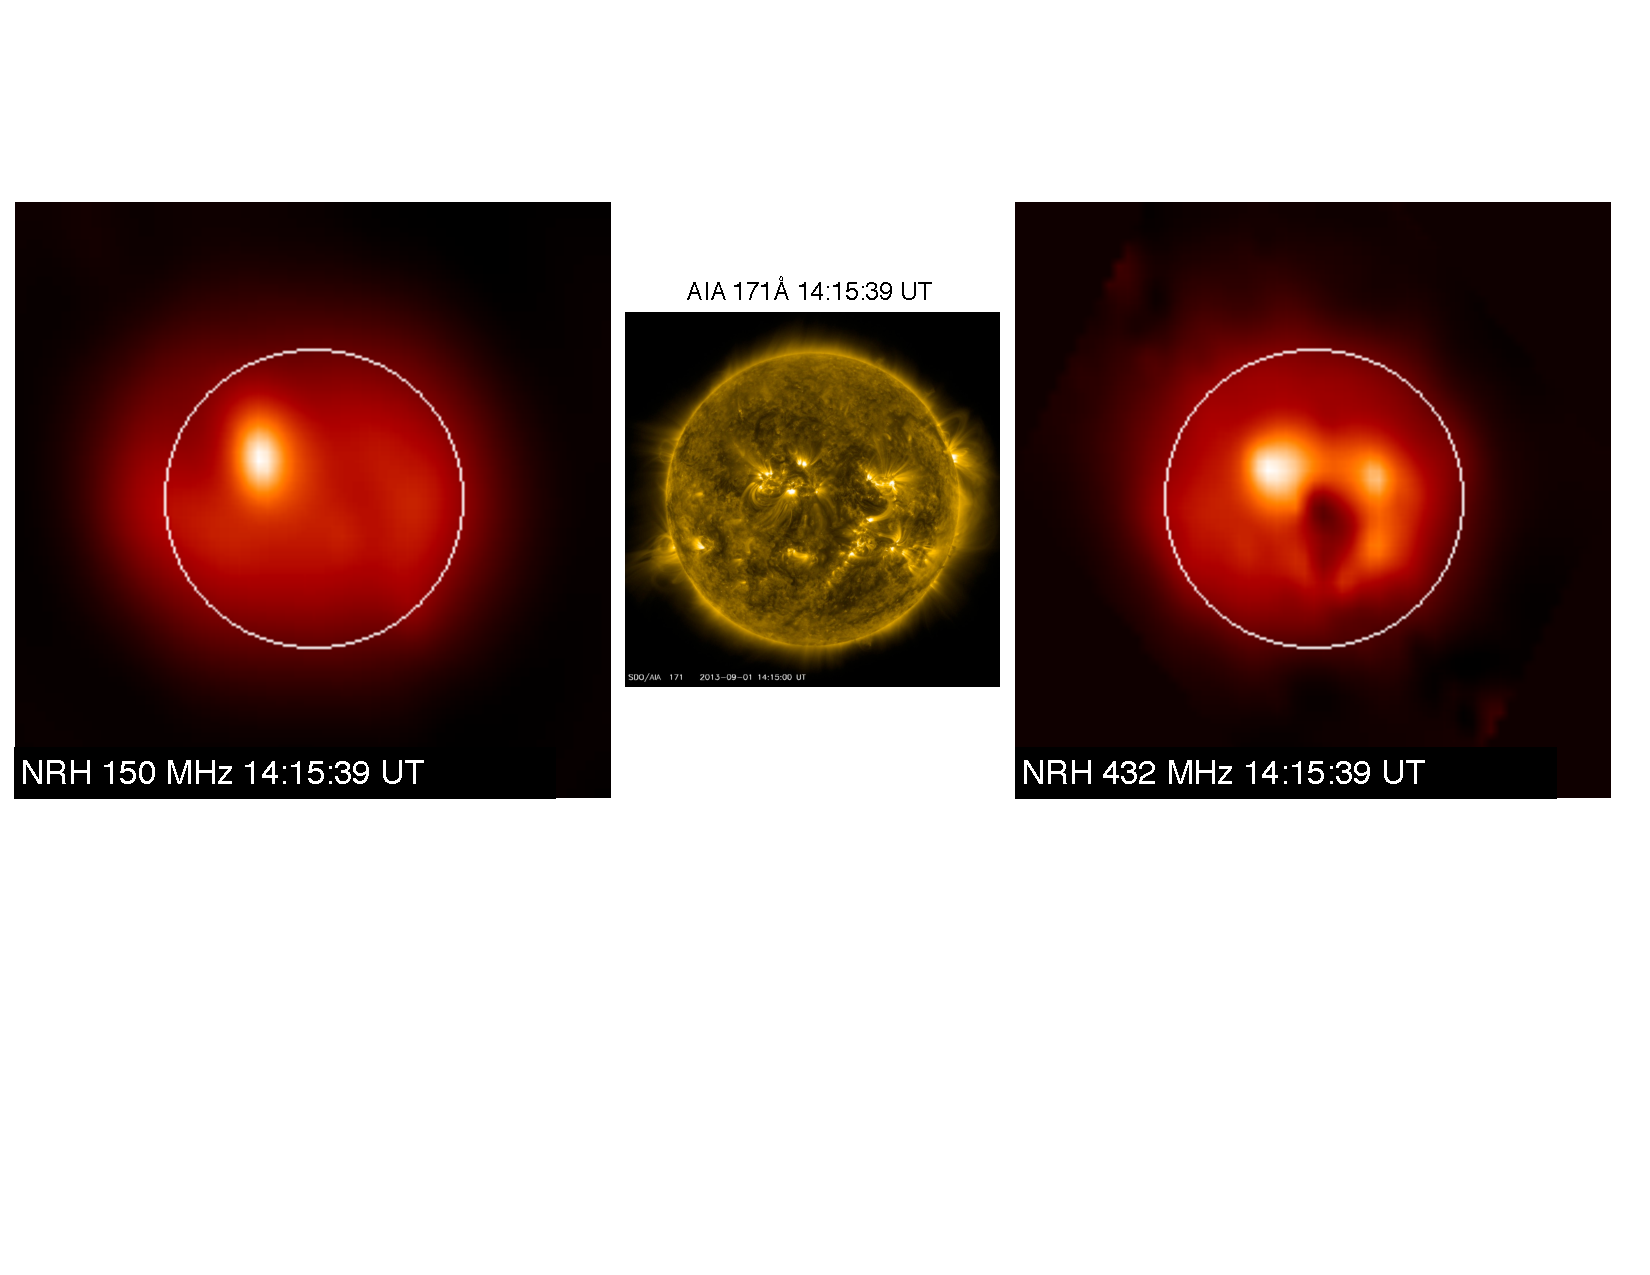
\includegraphics[scale=0.55, trim=0.5cm 7cm 0cm 2.5cm]{aia_nrh_compare.pdf}
\caption[NRH observations]{Observations from NRH at 150\,MHz and 432,MHz, with AIA\,171\,\AA~for comparison. All three images were taken at the same time at 14:15 UT on 01 September 2013.}
\end{center}
\end{figure}



\subsection{Nan\c{c}ay Decametric Array}\label{sec:32}

The Nan\c{c}ay Decametric Array consists of 72 ($6\,\mathrm{east} \times12\,\mathrm{west}$)conical antennas consisting of a left-handed helically wound component and a right handed helical component -- this makes the array contain 144 antennas in total, comprising 8000\,m$^2$ effective aperture at 30\,MHz \citep{lecacheux2000}. Each helix antenna is made of eight copper-steel wires wound on the surface of a cone and connected to the output coaxial cable by diode switches; only six wires are used at a time to form the antenna; the other two, diametrically opposite, are left disconnected. By changing the connections through the diode switches, the antenna can be electrically rotated around the cone axis, corresponding to a phase change of the antenna by steps of 45$^{\circ}$. The antennas are broadband (20--120\,MHz), low gain (low directivity) with a half power beam width of 90$^{\circ}$ centered on the cone axis \citep{boischot1980}. The entire array is steerable by phase delays withtin the 90$^{\circ}$  beam width of the individual antennas resulting in a possible tracking time of $\pm$4\,hr around the meridian, within a declination range of $-20^{\circ}$ to $+50^{\circ}$ .

The backend of the array consists of three possible receivers. The decametric activity consists of a wide-band swept-frequency analyzer which operates 400 channels between 20-90\,MHz. Left and right hand circular polarization are alternately sampled every 0.5 seconds from the left and right hand helical feeds of the antennas. The nominal operations for solar radio burst monitoring use this swept frequency receiver but there are other more sophisticated receivers available such as spectro-polarimeter with 1\,ms time sampling over providing 1024 channels and with a 60\,dB dynamic range. However, it has only a 12.5\,MHz instantaneous band, which is not so useful for solar radio burst monitoring.
\begin{figure}[!t]
\begin{center}
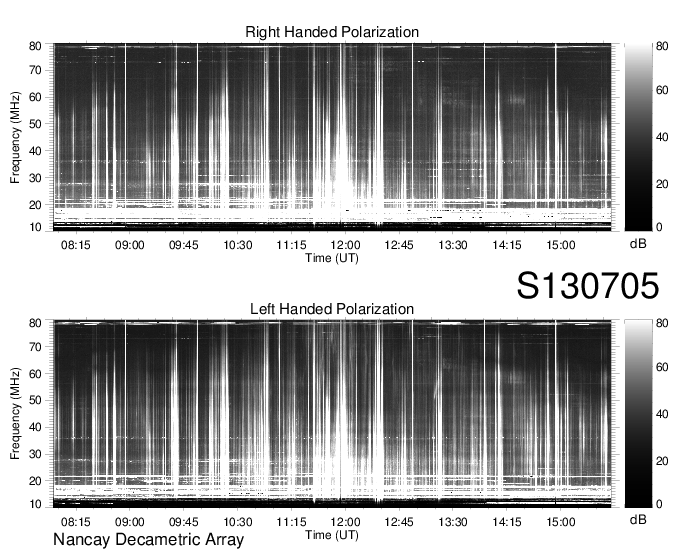
\includegraphics[scale=0.6]{S130705.png}
\caption[Nan\c{c}ay Decametric Array observations]{Nan\c{c}ay Decametric Array observations of an active period of type III radio bursts on 07 May 2013. Image courtesy of the {\it http://secchirh.obspm.fr/survey.php}}
\end{center}
\end{figure}

\subsection{STEREO WAVES}\label{sec:31}

Below this frequencies of $\sim$10\,MHz the Earth's ionosphere prevents the propagation of radio waves, hence radio emission below this frequency cannot be observed from ground-based observatories. To overcome this problem, there are a number of space based instruments that observe frequencies in the deca and kilometric wavelength ranges; the STEREO A and B spacecraft each carry such an instrument, known as STEREO WAVES or S/WAVES \citep{bougeret2008}. This instrument directly inherits it's design from the Ulysees \citep{stone1992}, Wind \citep{bougeret1995}, and Cassini \citep{gurnett2004} spacecraft.

The antenna system on each STEREO spacecraft consists of three mutually orthogonal 6-meter Beryllium-Copper monopole elements \citep{bale2008}, Figure~\ref{fig:swaves_antennas}. The elements diameter at the base is 1\,inch and tapers to 0.6\,inches at the tip. The three monopoles are each connected to a low noise and high impedance preamplifiers. The three preamplifiers each feed a number of receiving systems including the Fixed Frequency Receiver (FFR), the Time Domain Analyzer (TDS), and two frequency domain analyzers known as the Low Frequency Receiver (LFR) and High Frequency Receiver (HFR); only the LFR and HFR are described here.
\begin{figure}[!t]
\begin{center}
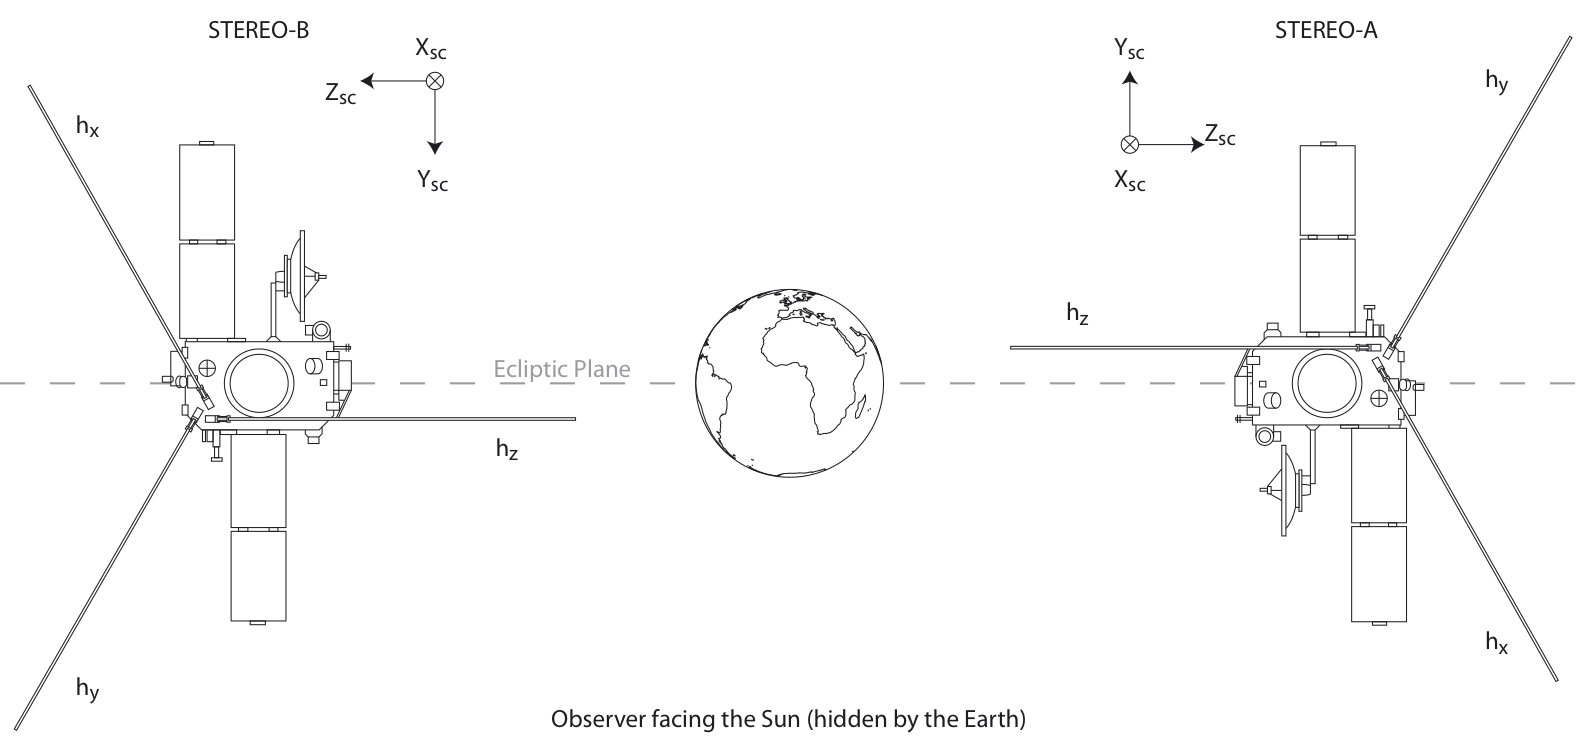
\includegraphics[scale=0.5]{Stereo-antennas.png}
\caption[The SWAVES antennas]{Configuration of the STEREO/WAVES antennas as seen from the Sun-Earth line, facing the Earth. Each monopole is 6\,m long and feeds a number of receiving instruments.}
\label{fig:swaves_antennas}
\end{center}
\end{figure}

The LFR is s direct conversion receiver that performs dynamic spectral analysis in the 2.5--160\,kHz band. The signal fed from the antennas and pre-amp is passed through a wavelet-like transform to perform digital spectral analysis in three 2-octave bands which each have 16 logarithmically spaced frequency channels (resulting in 48 log spaced channels in the 2.5--160\,kHz range). Receiver automatic gain control (AGC) ensures a high dynamic range of 120\,dB. Various combinations of the three antenna elements can be made to produce pseudo-dipole or monopole configurations. The signal is then 12-bit digitized and sent to a Digital Processing Unit (DPU)

The HFR is a dual sweeping receiver operating in the frequency range 125 kHz--16.025 MHz. It uses a super-hetereodyne technique to down-convert the signal frequencies to odd multiples of 25\,kHz that specifically avoid lines of noise that are generated by the spacecraft power supply, which may produce harmonic multiples of 50\,kHz. Due to the down-conversion process the HFR frqeuency range is covered in multiple steps of 50\,kHz increments, thus the highest spectral resolution is 50\,kHz. It has a dynamic range of 80\,dB. Like the LFR, it can receive various combinations of the three antenna elements in dipole or monopole modes. The signal is digitized by the same DPU as the LFR.

The time domain resolution for both the LFR and HFR is determined by the DPU. Nominal time resolution of the dynamic spectra produced by both receivers is 1\,minute.
\begin{sidewaysfigure}
\centering
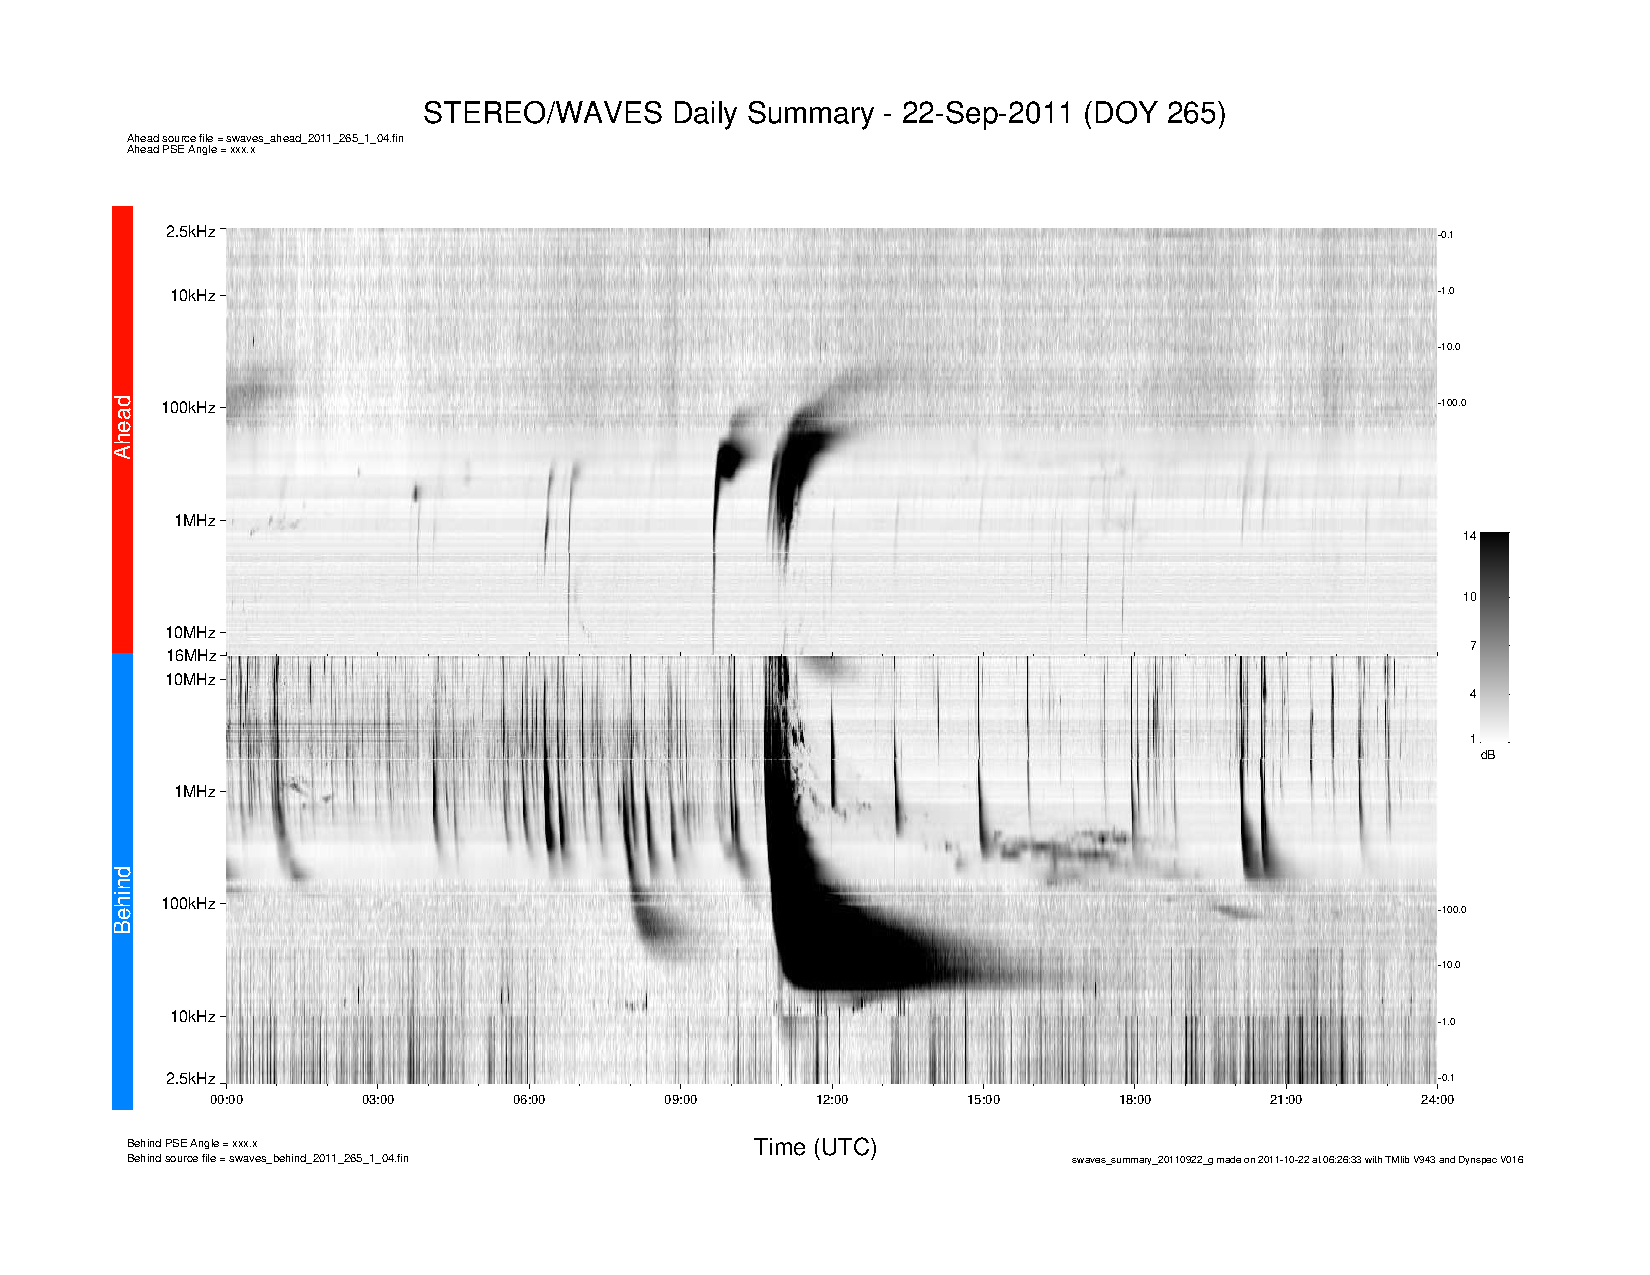
\includegraphics[scale=0.8, trim=0cm 2cm 0cm 2cm]{swaves_summary_20110922}
\caption[STEREO WAVES observations]{STEREO WAVES observations from the Ahead and Behind spacraft from 22 September 2011. A strong type III and interplanetary type II burst were observed by the Behind spacecraft. {\it Image courtesy of the STEREO Waves team http://swaves.gsfc.nasa.gov/.}}
\label{fig:swaves_antennas}
\end{sidewaysfigure}


\subsection{Rosse Solar Terrestrial Observatory}\label{sec:30}

\subsubsection{Antennas and Spectrometers}
The Rosse Solar Terrestrial Observatory was established in 2010 at Birr Castle, Co. Offaly Ireland (53$^{\circ}$ 05' 38.9'' , 7$^{\circ}$ 55' 12.7'') \citep{zucca2012}. The primary objective of the observatory is to observe low frequency radio bursts occurring in the Solar atmosphere and the ionospheric and geomagnetic response following this radio activity.  To date, three \textit{Compound Astronomical Low-cost Low-frequency Instrument for Spectroscopy and Transportable Observatory} (CALLISTO) spectrometers have been installed, with the capability of observing in the frequency range 10--870~MHz. The receivers are fed simultaneously by biconical and log-periodic antennas. Nominally, frequency spectra in the range 10--400 MHz are obtained with 4 sweeps per second over 600 channels. The instrumental set-up is described here.

RSTO employs three callisto receivers that cover the ranges of $10-100$, $100-200$, $200-400$\,MHz, respectively. The $10-100$\,MHz receiver (Callisto-1), is fed (via frequency up-converter) by a biconical Schwarzbeck antenna, model number VHBD 9134. The antenna elements are 4\,m long allowing a nominal frequency bandwidth of $20-200$\,MHz. Signal feed from the bicone to Callisto-1 is via $70\,\Omega$ coaxial cable, $\sim$20 meters in length Figure~\ref{fig:rsto_layout}. The bicone is mounted on a Yaesu-1 motor that permits solar tracking in the azimuth direction only (the antenna beam is symmetric in elevation). The bicone motor control unit (MCU) is located in the control room and PC communicates with the motor is via RS232 ($\sim20$\,m).
\begin{sidewaysfigure}
    \centering
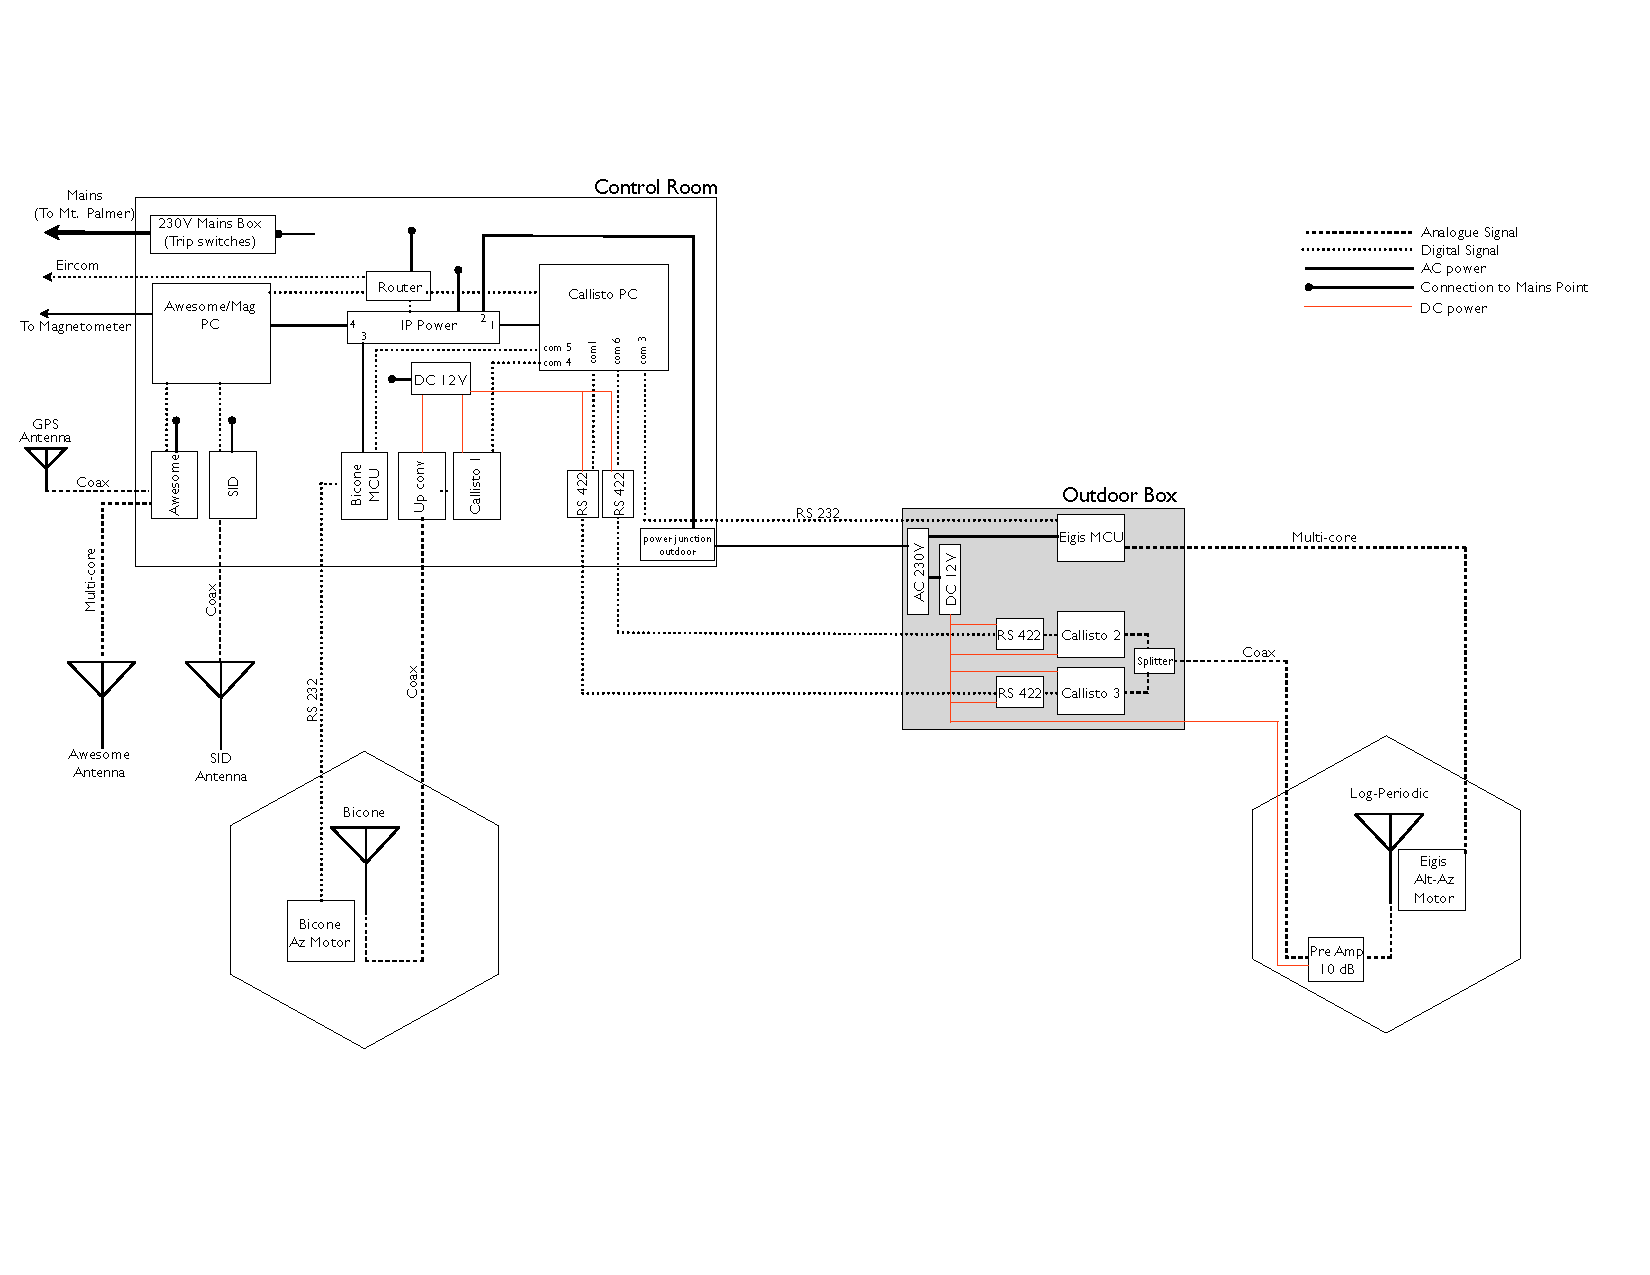
\includegraphics[scale=0.8, trim=0cm 3cm 1cm 2cm]{callisto_layout.pdf}
\caption[RSTO Instrumental Setup]{The Rosse Solar Terrestrial Observatory instrument and communications lay-out.}
\label{fig:rsto_layout}
\end{sidewaysfigure}

The $100-200$ and $200-400$\,MHz (Callisto-2 and -3, repsectively) are fed by a Tennadyne T28 log-periodic antenna. The antenna has a frequency band of $50 -1300$\,MHz with a $\sim$50 degree half-power beam width (HPBW). Signal from the antenna is fed into a 10 dB pre-amplifier (custom made by Joe McCauley), and from the preamp into a signal splitter. The splitter then feeds Callisto-2 and Callisto 3, see Fig.~\ref{fig:rsto_layout}. The digitized data for these two receivers is sent to the control PC via four RS422 conversion units (two next to the receivers and two next to the control PC). RS422 because of the high baud-rate and length of the cables ($\sim30$\,m) i.e., there may be interrupts and losses over this path length so the signal is sent differentially. The log-periodic antenna is fixed to an Eigis Alt-Az motor with an EPS-103 control unit, allowing tracking of the Sun thoughout the day. This control by a control unit in the outdoor box and communicates with the motor via a multicore cable $\sim10$\,m in length. The motor control unit is operated by the PC, communications are sent between the two via RS232 ($\sim30$\,m).

Callisto spectrometers were designed and built in ETH Zurich to monitor solar radio bursts in a frequency range of $10 - 870$\,MHz \citep{Benz2005}. The receiver is composed of standard electronic components, employing a Digital Video Broadcasting-Terrestrial (DVB-T) tuner assembled on a single printed circuit board. The number of channels per frequency sweep can vary between 1 and 400, with a maximum of 800 measurements per second. An individual channel has a 300\,kHz bandwidth during a typical frequency sweep of 250\,ms, and can be tuned by the control software in steps of 62.5\,kHz to obtain a more detailed spectrum of the radio environment. The narrow channel width allows for the measurement of selected channels that avoid known bands of radio interference from terrestrial sources.

\subsubsection{Nominal Operations}

The system is controlled by a Dell Vostro, Intel core i5. This control PC allows the system to be completely automated and stand alone, without the need for an on-site observer. Automatic nominal daily operations include (i) commence data recording of all three Callistos at 04:00\,UT, (ii) begin antenna solar tracking at sunrise, (iii) at 10 minutes past every hour the data is processed, background subtracted, and images are produced for online display at www.rosseobservatory.ie, (iv) at mid-day a high frequency resolution (62.5\,kHz) spectrum is taken, (v) stop solar tracking at sunset, (vi) archive the data products of the entire day (archive accessible online). This fully automated system is stable and requires maintenance or check up only every 6 or more months. If the system stops recording data the administrators are alerted by email. The entire automated process is carried out by a combination of Callisto GUIs, dedicated solar tracking GUIs, DOS Shell scripts, and IDL scripts.

The entire system is remotely accessible from Trinity College Dublin via a virtual desktop `VNC' software. The system may be remotely configured and nominal operations changed at any time. Should the system crash, a remote power recycling facility is available using an IP power board with its own web address, accessible from any web browser. Automated steps (i)-(vi) are recovered and begin automatically upon power recycling.

\subsubsection{Dynamic spectra from RSTO}

Since the installation of RSTO in September 2010 there has been a number radio bursts detected. The burst vary in their type, duration, and level of fine structure. The observatory has been successful in picking up type I storms, type IIs, type IIIs, a number of herringbone observations, and type V and VI. Some samples of these are given in Figures~\ref{fig:typeII_hb} to~\ref{fig:type_III}, with further dynmaic spectra in the Appendix.
\begin{figure}[!t]
\begin{center}
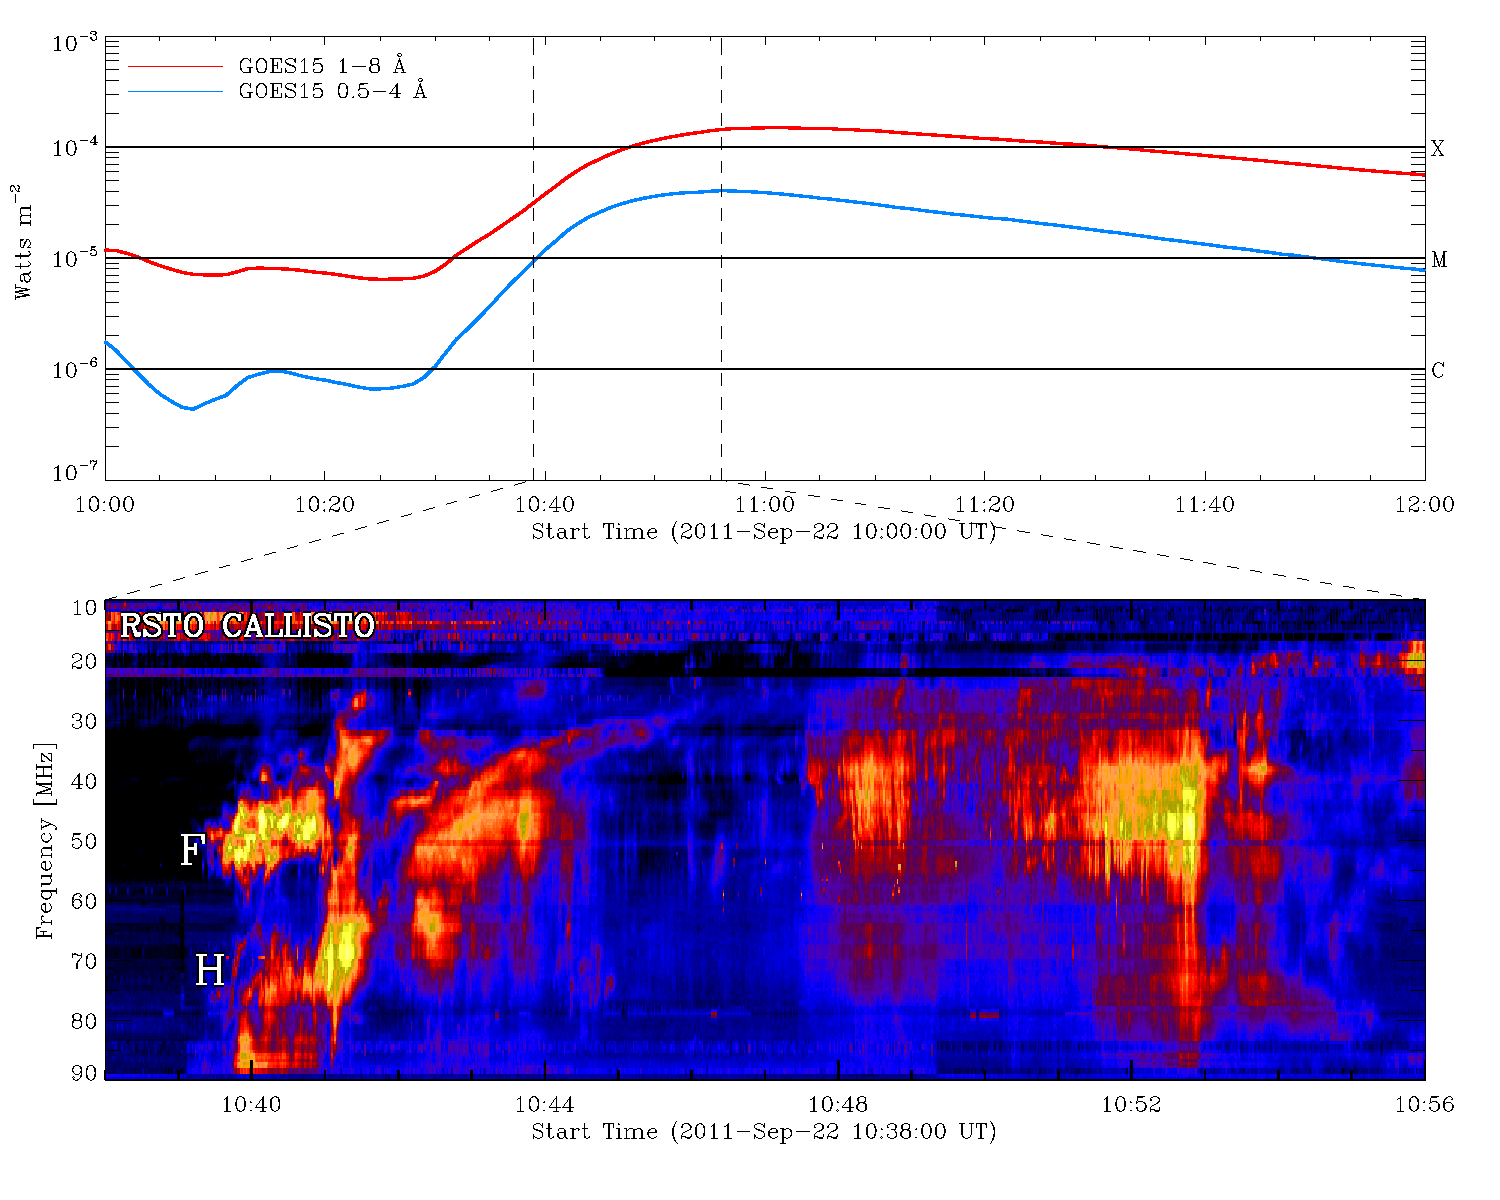
\includegraphics[scale=0.62, trim=1cm 0cm 0cm 0cm]{20110922_typeII_hb.pdf}
\caption[Callisto observations type II and herringbones]{A radio burst from 22 September 2011 observed at RSTO. This radio burt was detected by the 10--100\,MHz Callisto fed by the bicone antenna. The radio burst was quite complex, consisting of the fundamental and harmonic of a type II burst followed by herringbone fine structures. The top plot shows the GOES light curves for comparison, with the dashed vertical line indicating start and end times of the dynamic spectra.}
\label{fig:typeII_hb}
\end{center}

\end{figure}
\begin{figure}[!t]
\begin{center}
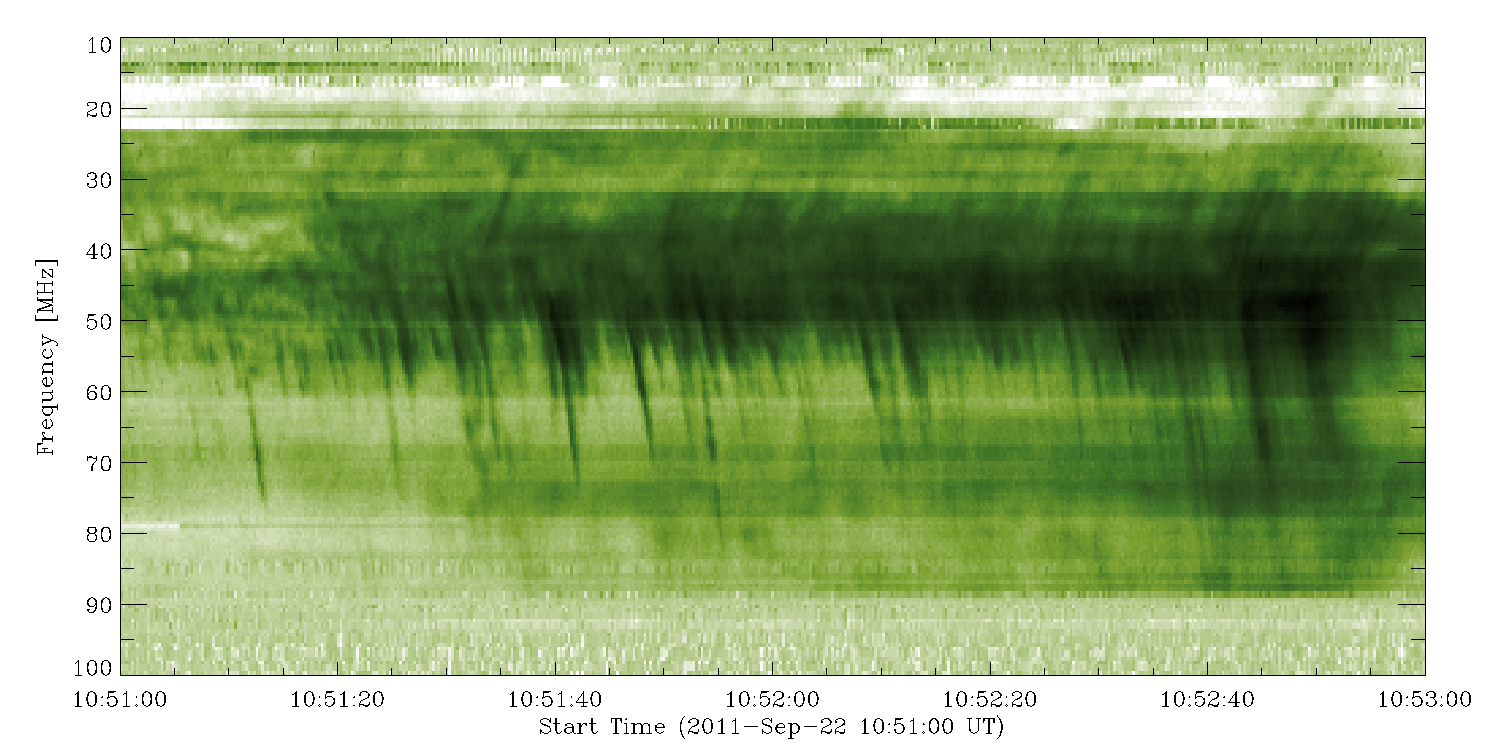
\includegraphics[scale=0.5, trim=1cm 0cm 0cm 0cm]{callisto_instr_paper2.pdf}
\caption[Callisto observations type II and herringbones]{A zoom of the herringbone structure shown in Figure~\ref{fig:typeII_hb}. The time sampling of the callisto spectrometers (0.25\,s) is fast enough to catch such herringbone features}
\label{fig:herringbones}

\end{center}
\end{figure}
\begin{figure}[!t]
\begin{center}
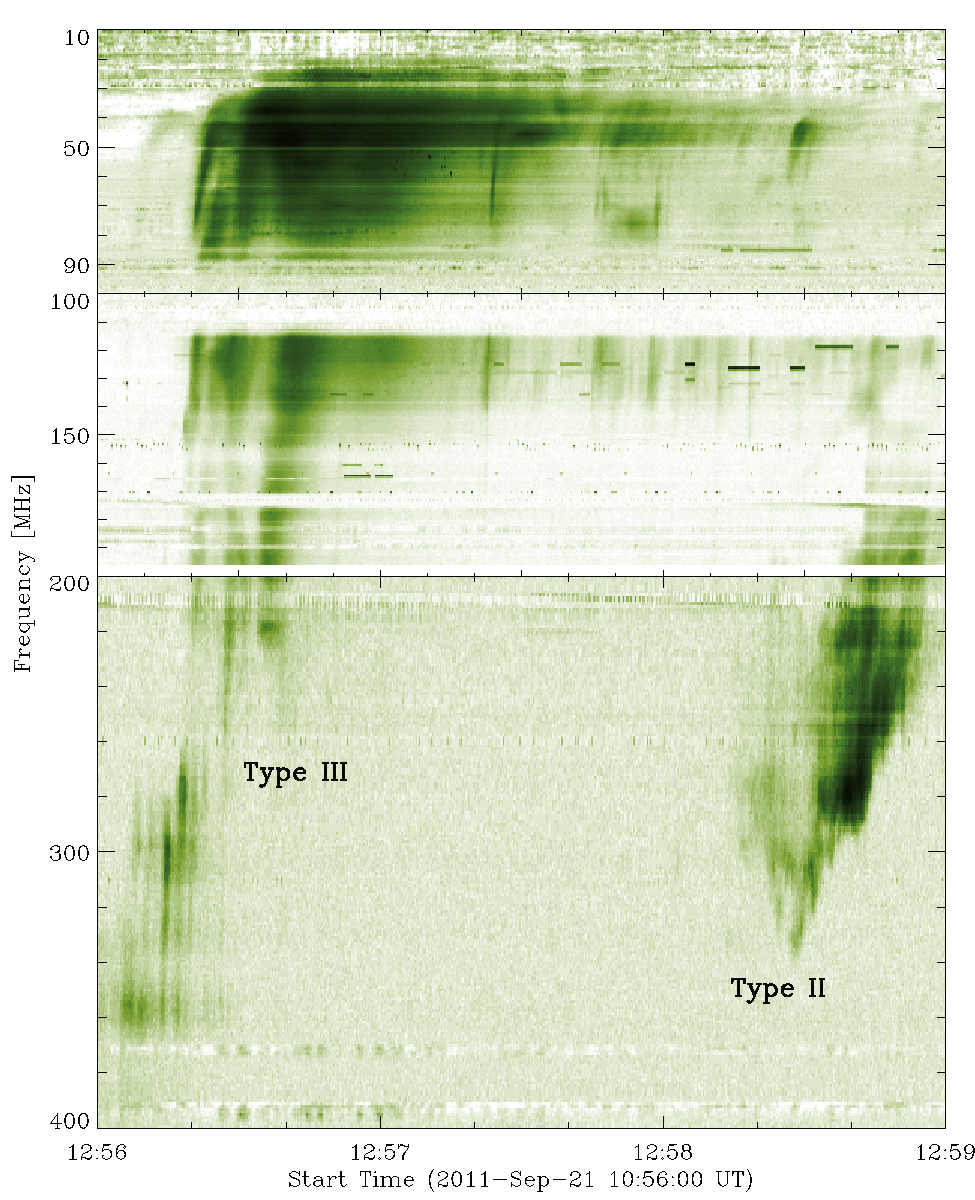
\includegraphics[scale=0.7, trim=1cm 0cm 0cm 1cm]{callisto_instr_paper3}
\caption[Callisto observations type II and herringbones]{A type III and II radio burst observed on 21 September 2011. This spectra demonstrates the low levels of RFI at RSTO, especially in the 200--400\,MHz range where there is almost no RFI.}
\label{fig:type_III}
\end{center}
\end{figure}


\subsubsection{eCallisto Network}
\begin{figure}[!t]
\begin{center}
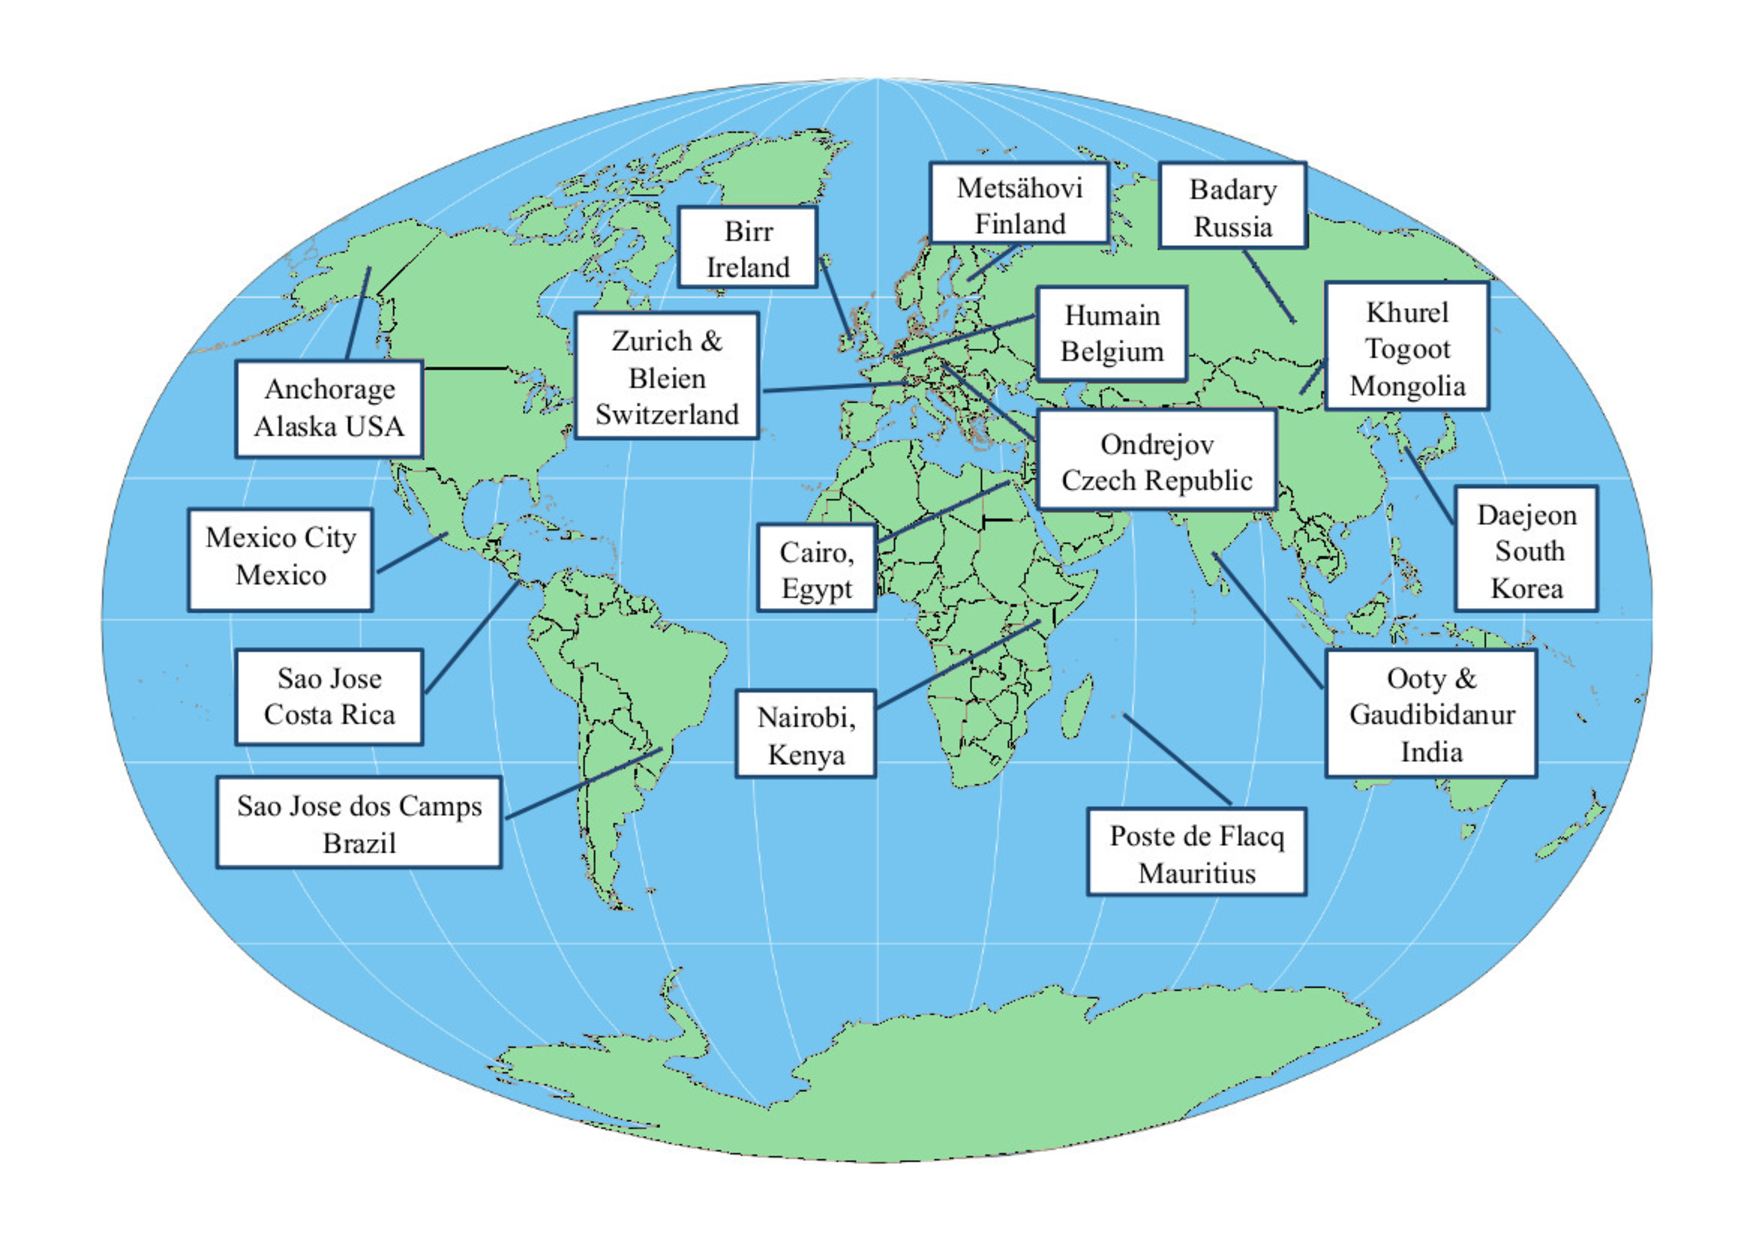
\includegraphics[scale=0.45]{callisto_worldwide.pdf}
\caption[Callisto Worldwide]{Worldwide distribution of Callisto sites, offering almost 24 coverage of solar radio activity at most latitudes.}
\label{fig:callisto_worldwide}
\end{center}
\end{figure}
%------------Describing Network and Low RFI----------------------%
RSTO is part of the e-Callisto network\footnote{www.e-callisto.org}. The network consists of a number of spectrometers located around the globe, and designed to monitor solar radio emission in the meter and decameter bands (\citealt{Benz2009}; Figure~\ref{fig:callisto_worldwide}).  Each of the instruments observes automatically, and data is collected each day via the Internet and stored in a central database at Fachhochschule Nordwestschweiz (FHNW), and operated by ETH Zurich\footnote{soleil.i4ds.ch/solarradio/CALLISTOQuicklooks/}. One of the important features of RSTO is the particularly low radio frequency interference (RFI) of the site. 
\begin{figure}[!t]
\begin{center}
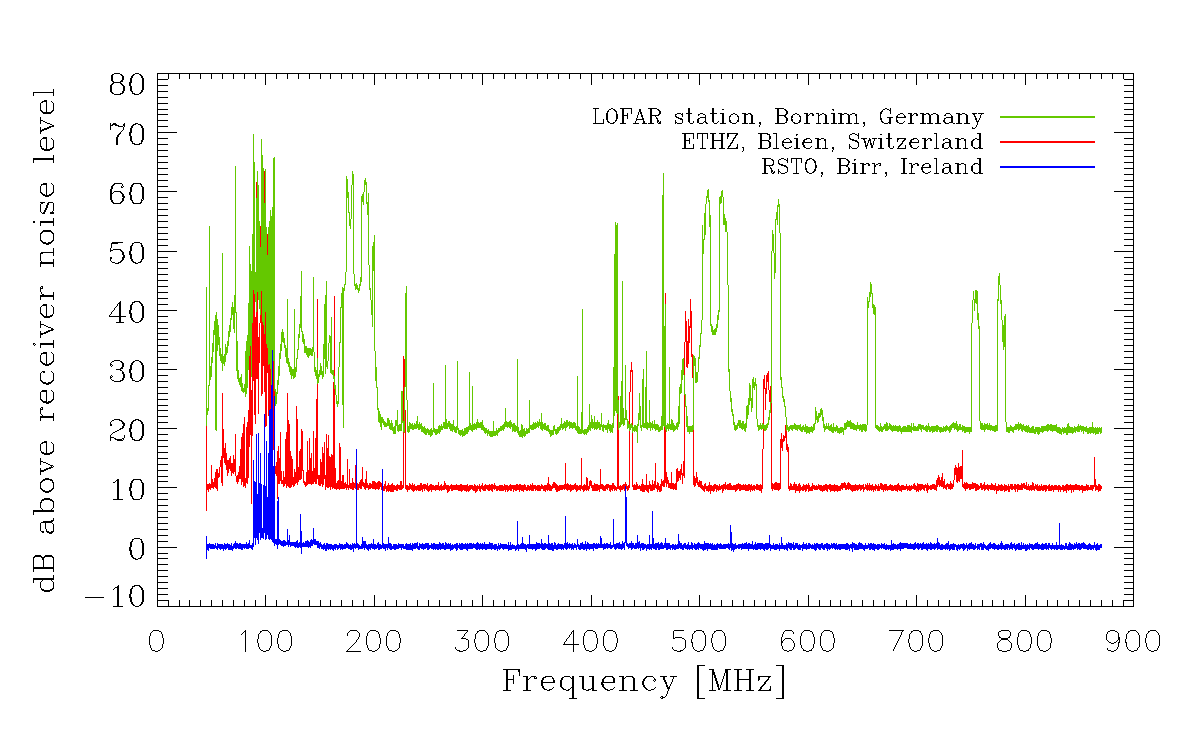
\includegraphics[scale=0.7]{rfi_survey.pdf}
\caption[RSTO RFI Survey]{Radio frequency survey from the RSTO in Birr Castle Demesne (blue), Bleien Radio Observatory in Switzerland (red; offset by 10 dB) and Potsdam Bornim (green; offset by 20 dB). The RSTO spectrum is quiet at all frequencies that were tested, except for the FM band covering 88--108 MHz. The surveys were conducted using the same equipment.}
\label{fig:rfi_survey}
\end{center}
\end{figure}

To compare RSTO to other radio observing sites, an survey of RFI at RSTO was performed in June 2009. The detected spectrum is shown in Figure~\ref{fig:rfi_survey}.  A commercial DVB-T antenna covering the range from 20~MHz up to 900~MHz was used for the survey, which was directly connected via a low-loss coaxial cable to a Callisto receiver with a sensitivity of 25~mV/dB. The channel resolution was 62.5~kHz, while the radiometric bandwidth was about 300 kHz. The sampling time was 1.25 ms per frequency interval, while the integration time was about 1~ms.  Figure~\ref{fig:rfi_survey} shows the RFI radio surveys of RSTO, Bleien Observatory in Switzerland, and the Potsdam LOFAR station in Germany. There is an high level of interference at 20--200~MHz for the Bleien and Potsdam sites, while the RSTO site has a low level of RFI.

\subsection{Dynamic Spectra Data Reduction}

The Nan\c{c}ay Decametric Array, STEREO WAVES, and the Callisto spectrometers each have basic data reduction techniques in common. The most basic of these is background subtraction. Analogous to the dark current on a CCD, there will be some background signal detected due to the system electronics. This is due to a number of effects including the any DC bias and the noise produce by system thermal properties. This background may be subtracted by a variety of techniques, such as averaging the dynamic spectrum through time and using this as a background, subtracting a spectrum occurring just before a detected radio burst, or automatically detecting a spectra with no radio burst and using this as a background. The last type is the one implemented on the dynamic spectra used in this thesis work. The procedure is implemented in the IDL procedure {\it constbacksub.pro}. This function firstly computes the average of each frequency channel in time and subtracts this from the original spectrogram. It then computes the standard deviation of each time-step. The time-steps containing a radioburst should have the largest standard deviation, while those without a burst will have small standard deviation. By default the smallest  5\% of the standard deviations is averaged and used as a background.

Dynamic spectra may also be contaminated by radio frequency interference (RFI). This may be sporadic, periodic and regular, or continuous in time. RFI is generally very difficult to remove from a dynamic spectra while still maintaining the desired signal (radio burst). The techniques of RFI removal may be a simple smoothing of the data  or convolution with a Gaussian to `average out' the signal. Much more sophisticated RFI identification algorithms are based on multiscale filtering of the dynamic spectra image or using a kurtosis estimator \citep{nita2007, nita2010}(RFI is generally much more `peaked' in either frequency or time). Generally, frequency channels with bad contamination by RFI are avoided if possible.

PUT IN PLOTS TO DEMONSTRATE THE ABOVE

